% ######################################################################
%
% 			PREAMBULE
%
% ######################################################################

% -------------------------------------------------------
% Ce document est un raport. cinquantaine de pages / plusieurs sections
% -------------------------------------------------------
\documentclass[a4paper,12pt]{report}

% -------------------------------------------------------
% Utiliser latin1 pour les accents
% ne pas utiliser utf8 et Latex n'aime pas utf8 ET latin1
%\usepackage[utf8]{inputenc}
% -------------------------------------------------------
\usepackage[utf8]{inputenc}

% utiliser plutôt french, frenchb est obsolete
\usepackage[T1]{fontenc}
\usepackage[english,french]{babel}

\usepackage{amsmath}
\usepackage{amssymb}
\usepackage{amsfonts}
\usepackage{array}
\usepackage{booktabs}
\usepackage{diagbox} % barre oblique pour les cellule à 2 entrées
\usepackage[pdftex]{graphicx}
\usepackage{hhline}
\usepackage{hyperref}
\usepackage{lmodern}
\usepackage{multicol}
\usepackage{subcaption}
\usepackage{supertabular}
\usepackage{textcomp}
\usepackage{xcolor}
\usepackage{xspace}
\usepackage{pdflscape}

% -------------------------------------------------------
% Pour utiliser certains symboles mathématiques (statistiques)
% -------------------------------------------------------
\DeclareMathOperator{\E}{\mathbb{E}} % Espérence / Expectation
\DeclareMathOperator{\V}{\mathbb{V}} % Variance  / Variance

% -------------------------------------------------------
% Annexes
% -------------------------------------------------------
\usepackage[toc,page]{appendix} 
\renewcommand{\appendixtocname}{Annexes}
\renewcommand{\appendixname}{{\sffamily Annexe}} 

% -------------------------------------------------------
% Ajout LP
% -------------------------------------------------------
\usepackage{todonotes}

% -------------------------------------------------------
% Théorèmes
% -------------------------------------------------------
\usepackage{amsthm}
\theoremstyle{plain}				% Choix du style
\newtheorem{theoreme}{Théorème}	% Définition de l'environnement 1
\newtheorem{example}{Exemple}
\theoremstyle{definition}				% Choix du style
\newtheorem{definition}{Définition} %[section]	% Définition de l'environnement définition

% -------------------------------------------------------
% Pour les ALGORITHMES
% linesnumbered	: les lignes sont numérotées
% ruled			: Le caption est en haut et bordé de lignes horizontale
% vlined		: Regroupement des bloc d'instructions par ligne verticales
% -------------------------------------------------------
\usepackage[linesnumbered, ruled, vlined, french]{algorithm2e}

% Commandes en français:
\SetKwInput{KwRes}{R\'esultat}%
\SetKw{WEntree}{\textcolor{red}{Entrée}}
\SetKw{WEntrees}{\textcolor{red}{Entrées}}
\SetKw{WSaisir}{Saisir}
\SetKw{WInitialisation}{\textcolor{red}{Initialisation}}
\SetKw{WTraitement}{\textcolor{red}{Traitement}}
\SetKw{WAssigne}{\textcolor{blue}{prend la valeur}}
\SetKw{WSortie}{\textcolor{red}{Sortie}}
\SetKw{WSorties}{\textcolor{red}{Sorties}}
%
\SetKwIF{Si}{SinonSi}{Sinon}{Si}{alors}{sinon si}{sinon}{fin si}
\SetKwFor{Tq}{Tant que}{faire}{fin tantque}
\SetKwFor{Pour}{Pour}{faire}{fin pour}
\SetKw{WAfficher}{Afficher}
\SetKwRepeat{Repeter}{répéter}{jusqu'à}%
%
\SetKw{Return}{\textcolor{red}{Renvoyer}}%
%
\SetKwProg{Init}{init}{}{}
% mettre les commentaire des algos en bleu

% -------------------------------------------------------
% Pour les ALGORITHMES façon PYTHON
% -------------------------------------------------------
\usepackage{listings}
\lstset{literate={á}{{\'a}}1 {é}{{\'e}}1 {í}{{\'i}}1 {ó}{{\'o}}1 {ú}{{\'u}}1{Á}{{\'A}}1 {É}{{\'E}}1 {Í}{{\'I}}1 {Ó}{{\'O}}1 {Ú}{{\'U}}1{à}{{\`a}}1 {è}{{\`e}}1 {ì}{{\`i}}1 {ò}{{\`o}}1 {ù}{{\`u}}1{À}{{\`A}}1 {È}{{\'E}}1 {Ì}{{\`I}}1 {Ò}{{\`O}}1 {Ù}{{\`U}}1{ä}{{\"a}}1 {ë}{{\"e}}1 {ï}{{\"i}}1 {ö}{{\"o}}1 {ü}{{\"u}}1{Ä}{{\"A}}1 {Ë}{{\"E}}1 {Ï}{{\"I}}1 {Ö}{{\"O}}1 {Ü}{{\"U}}1{â}{{\^a}}1 {ê}{{\^e}}1 {î}{{\^i}}1 {ô}{{\^o}}1 {û}{{\^u}}1{Â}{{\^A}}1 {Ê}{{\^E}}1 {Î}{{\^I}}1 {Ô}{{\^O}}1 {Û}{{\^U}}1{œ}{{\oe}}1 {Œ}{{\OE}}1 {æ}{{\ae}}1 {Æ}{{\AE}}1 {ß}{{\ss}}1{ű}{{\H{u}}}1 {Ű}{{\H{U}}}1 {ő}{{\H{o}}}1 {Ő}{{\H{O}}}1{ç}{{\c c}}1 {Ç}{{\c C}}1 {ø}{{\o}}1 {å}{{\r a}}1 {Å}{{\r A}}1{€}{{\EUR}}1 {£}{{\pounds}}1}

\lstdefinestyle{stylepython}{
	language=Python,
	basicstyle=\ttfamily,
	commentstyle=\color{red},
	keywordstyle=\color{blue},
	stringstyle=\color{green}, %olive
	numberstyle=\tiny,numbers=left,
	stepnumber=1,numbersep=5pt}

% -------------------------------------------------------
% Information PDF généré
% -------------------------------------------------------
\hypersetup{pdftex, colorlinks=true, linkcolor=blue, citecolor=blue, filecolor=blue, urlcolor=blue, pdftitle=, pdfauthor=Florian Colas, pdfsubject=, pdfkeywords=}

% -------------------------------------------------------
% MACRO
% -------------------------------------------------------
% Pm||Cmax
\newcommand\problemGrahamPm{$P_m||C_{\max}$\xspace}
% P2||Cmax
\newcommand\problemGrahamPII{$P_2||C_{\max}$\xspace}	%apparemment ne supporte pas les chiffres.
% P||Cmax
\newcommand\problemGrahamP{$P||C_{\max}$\xspace}
% Cmax
\newcommand\cmax{$C_{\max}$\xspace}

% Della Croce et Scatamacchia \textnormal{
\newcommand\dcs{Della Croce et Scatamacchia\xspace}

% -------------------------------------------------------
% Dossier des figures
% -------------------------------------------------------
\graphicspath{{./fig/}}

% -------------------------------------------------------
% Ajout L. Philippe
% Utilisation des Todo inline en macro --> tdi
% -------------------------------------------------------
\usepackage{todonotes}
\newcommand{\tdi}[1]{\todo[inline]{{#1}}{}}
\newcommand{\lp}[1]{\todo[author=LP,color=yellow,inline]{#1}}
\newcommand{\lcc}[1]{\todo[author=LCC,color=green,inline]{#1}}
\newcommand{\fco}[1]{\todo[author=FCO,color=teal,inline]{#1}}
\newcommand{\jb}[1]{\todo[author=JB,color=orange,inline]{#1}}

% -------------------------------------------------------
% Information générales (en attendant la page de garde)
% Utilisé par \maketitle
% -------------------------------------------------------
\title{Évaluation d'algorithmes d'ordonnancement}
\author{Florian Colas}
\date{\today}

% ######################################################################
%
% 				DOCUMENT
%
% ######################################################################
\begin{document}

% #######################################################
% Numérotation des pages
% #######################################################
\pagenumbering{roman}

% =======================================================
% Page de garde
% Utilise Information générales
% Ecrit le titre + auteur + date
% =======================================================
\maketitle

\section*{Dédicaces} \label{sec:dedicace}
je dédie....

\section*{Remerciements} \label{sec:remerciements}
je remercie....

% -------------------------------------------------------
% Table des matières
%
% On renomme en Sommaire (document français)
%
% On définit la profondeur de la table des matières
% -1 partie,    0 Chapitre,
% 1 Section,    2 sous sections,  3 sous sous section
% 4 Paragraphe, 5 Sous paragraphe
%
% Les sections sont numérotées 1 2 3
% -------------------------------------------------------
\renewcommand{\thesection}{\arabic{section}}
\renewcommand{\contentsname}{Sommaire}
\setcounter{tocdepth}{3}	% avant 2 pour la table des matières
\setcounter{secnumdepth}{3}	% pour les section sous et sous sous et paragraphes
\tableofcontents


\bigskip

% #######################################################
% Numérotation des pages
% #######################################################
\pagenumbering{arabic}

\lp{Attention aux majuscules/minuscules dans les listes et après :}
% =======================================================
% 1 INTRODUCTION GENERALE
% =======================================================
\section{Introduction générale} \label{sec:introductionGenerale}

% -------------------------------------------------------
% du plus général Ordonnancement et traitement parallèle 	>
% au plus spécifique P||Cmax vers ouverture					<
% -------------------------------------------------------

% ORDONNANEMENT
La question d’ordonnancement est omniprésente, dans la vie pratique, l'industrie, le transport, 
  les institutions, la santé et toute autre discipline qui nécessite une organisation.
  L'ordonnancement consiste à agencer au mieux des tâches, des jobs reliés ou non entre eux 
  pour atteindre un but, tout en optimisant un critère particulier. 
Dans la construction d'une maison, depuis la pose de la première dalle jusqu'à la pose du dernier carrelage, 
  tout a été organisé pour réduire au maximum le retard total. 
  Certaines tâches ont pu être effectuées en parallèle (pose de la plomberie, pose de l'électricité), 
  quant à d'autres elles n'ont pu commencer qu'après l'achèvement d'ouvrages 
  (pose des tuiles après la finalisation de la charpente). 

% ORDONNANEMENT dans l'informatique
L’ordonnancement intervient aussi dans l'attribution et l'ordre d’exécution des jobs à réaliser par processeur. 
Même pour une machine mono-processeur, l'ordre a son importance si des jobs sont liés par des relations de précédences. 
% ORDONNANEMENT dans l'informatique parallèle
La question est d'autant plus essentielle depuis l'apparition des ordinateurs à structure parallèle.
En effet, la composition d'un ensemble de jobs sur plusieurs microprocesseurs, même sans lien entre eux, a des répercutions sur le temps total nécessaire pour exécuter tous ces jobs. 

% Parallélisme
Le parallélisme est un type d'architecture informatique dans lequel plusieurs processeurs exécutent 
  ou traitent une application, un calcul simultanément. 
Cette structure aide à effectuer de grands calculs en divisant la charge de travail entre plusieurs 
  processeurs capables de communiquer et de coopérer.     

% Scheduling
Le calcul de l'attribution de chaque tâche d'un ensemble de jobs aux ressources disponibles dans le but d'optimiser un critère est lui-même un job.  \jb{Je ne comprends pas la fin de la phrase précédente}
Ce calcul est appelé algorithme d'ordonnancement (Scheduling algorithm). 
Celui-ci doit être effectué le plus rapidement possible et donner la réponse d'ordonnancement en 
  adéquation avec ce qui est attendu.


% Scheduling et P||Cmax
Un cas particulier et fréquent d'ordonnancement est le problème \problemGrahamP tel que définit 
  dans la classification à trois champs de Graham \emph{et al.} \cite{graham1979optimization}. 
Le but de \problemGrahamP consiste à planifier un ensemble $J=\{j_1, j_2, \ldots, j_n\}$ de 
  $n$ jobs (ou tâches) indépendants, 
  sur $m$ machines identiques,  
  dans le but d'optimiser le temps total de traitement appelé makespan (noté $C_{max}$).
Le temps nécessaire de réalisation de chaque job $p_i$ $\in P=\{p_1, p_2, \ldots, p_n\}$  
  (avec $1 \leq i \leq n)$ est connu à l'avance. 
Un job commencé est complété sans interruption (non préemptif), 
  et est exécuté par une seule machine. 
Une machine ne traite qu'un seul job à la fois. 

% problématique générale 
Mais, comme l'ont démontré Garey et Johnson, 
  \problemGrahamPII avec $m = 2$ est un problème NP-Difficile \cite{garey1978strong}, et 
  \problemGrahamP avec $m \geq 3$ est un problème NP-Difficile au sens fort \cite{garey1982computers}.
En plus, \problemGrahamP devient un problème NP-Difficile, du moment que le nombre de machines 
  est fixé \cite{chen1999potts}, comme l'a montré Rothkopf \cite{rothkopf1966scheduling} qui a 
  présenté un algorithme de programmation dynamique.\fco{voir le type d'algo pseudo-polynomial ?}

Donner la solution optimale à un problème d'ordonnancement \problemGrahamP n'est pas réaliste. \jb{J'ajouterais «Dans le cas général»}
La résolution de celui-ci demanderait un temps excessif et donc rédhibitoire.
Comme les machines sont identiques, et travaillent à la même vitesse, la difficulté repose uniquement 
  sur le regroupement des jobs.
La résolution de ce problème d'ordonnancement va reposer sur des méthodes d'approche qui consistent à 
  calculer en temps polynomial une solution ``assez'' proche de la valeur optimale.

Les jobs sont exécutés sans interruption ni coupure. Donc, le makespan ne peut pas être inférieur à 
  la taille du jobs le plus long i.e. $(\max_i\{p_i\})$.
  Il ne peut pas être inférieur non plus à la moyenne des tailles des jobs par machine
  i.e. $\frac{1}{m} \sum_{i=1}^{n} p_i$.
Donc toutes les solutions ont une borne minimale \cite{mcnaughton1959scheduling}: \\

  \begin{center}
  $\text{borne}_{min} = \max \{ \max_i\{p_i\}, \frac{1}{m} \sum_{i=1}^{n} p_i \}$
  \label{borneMini}
  \end{center}

L'existence d'une solution qui résout efficacement le problème de manière optimale
  n'est pas pensable, à moins que $P = NP$.
Dans la littérature, l'étude d'ordonnancement est très riche et abondante. 
Le but étant d'améliorer le temps de calcul, et d'approcher le résultat optimal. 
Les solutions proposées sont des heuristiques, ou des approximations.

Le but d'une heuristique (du grec \emph{heuriskein}: trouver) est 
  de produire une solution respectant les contraintes du problème et 
  de bonne qualité selon le critère d'optimisation considéré. 
La solution ne sera pas forcément optimale mais une heuristique efficace tente de trouver une 
  solution de bonne qualité suivant le temps de résolution imparti.
Ces algorithmes calculent des solutions, dont la borne maximale, au pire des cas n'est pas maîtrisée: 
une étude du comportement est nécessaire pour définir cette borne maximale.  
Pour chaque étude de comportement, les notions suivantes sont utilisées :

\begin{itemize}
% RESULTAT DE L'ALGORITHME A
\item $C_m^A(J)$ Le résultat (makespan) de l'ordonnancement
	d'un ensemble $J$ de jobs,
	sur $m$ machines parallèles, identiques,
	obtenu par l'algorithme~$A$.
% RESULTAT OPTIMAL
\item $C_m^\star(J)$ Le makespan optimal, idéal, de l'ordonnancement
	d'un ensemble $J$ de jobs,
	sur $m$ machines parallèles identiques.
% RATIO OBTENU/OPTIMAL
\item $\Gamma(A)=\frac{C_m^A(J)}{C_m^\star(J)}$
	Le ratio d'approximation atteint par l'algorithme $A$ au pire cas.
\end{itemize}
   
Parfois, cette borne est arbitrairement large et n'a pas été analysée. Une simulation permet d'obtenir des 
  informations générales sur les tendances.
Parmi les heuristiques les plus étudiées, nous pouvons citer 
  LPT (Longest Time Processing) \cite{graham1966bounds}, 
  LDM (Largest Differencing Method) \cite{karmarkar1982differencing}, 
  COMBINE \cite{lee1988multiprocessor}.
  
\bigskip
%--------------------------------------
% génese du rapport
%--------------------------------------
Ce mémoire prend le texte de \dcs \cite{della2020longest} comme point de départ.    
Ces derniers revisitent l'heuristique LPT en appliquant aux données d'entrée du problème une stratégie gloutonne. 
L'algorithme développé appelé SLACK devient très compétitif par rapport à d'autres heuristiques, 
  tant en complexité en temps qu'en ratio d'approximation. 
Cette conclusion est le résultat d'un protocole expérimental défini dans \cite{iori2008scatter}. 
Les algorithmes sont testés sur des instances basées sur 2 types de générations de nombres pseudo-aléatoires, contenant 10, 50, 100, 500 et 1000 jobs, à planifier sur 5, 10 et 25 machines. 
Pour $n > m$ cela représente 13 points de comparaisons qui permettent aux auteurs de déclarer SLACK comme étant une alternative sérieuse à LPT, LDM et COMBINE. 
Ce résultat est intéressant. En effet la borne d'approximation se rapproche un peu plus de l'optimal. 
Mais ce résultat empirique repose sur un nombre assez restreint d'échantillons. Sont-ils assez représentatifs pour en dégager une conclusion absolue ? Est-ce le comportement général de SLACK (ou tout autre algorithme) d'être le plus efficace s'il l'est pour ces 13 points ? 

Le but de ce document est de répondre à cette question, à l'aide des démarches suivantes :

\begin{itemize}
	\item Reproduire le protocole expérimental de \dcs.  
	\item \'{E}largir ce protocole expérimental à d'autres types de générations aléatoires, 
	voire à de vraies archives de listes de tâches, et à un spectre plus large de nombres de jobs et de machines.  
\end{itemize} 

\bigskip
% -------------------------------------------------------
%PLAN
% -------------------------------------------------------
\fco{a revoir}
\lp{Oui tu peux aussi ajouter ce qui a été dit par Julien, à savoir
  étendre aux principaux algos}
Le Chapitre suivant est un état de l'art au problème \problemGrahamP. La mise en place expérimentale et les choix effectués dans ce mémoire sont évoqués en chapitre 3. Puis nous aborderons la création des listes de temps et les instances dans le chapitre 4. Le chapitre 5 présente l'environnement de tests, avant d'aborder et présenter en chapitre 6 le résultat de la reproduction du protocole expérimental de \dcs et du protocole élargi. Ce document se termine par une discussion sur les protocoles de tests des heuristiques.

Les annexes abordent certains points importants de l'implémentation des algorithmes et de la création des listes de temps.  

% =======================================================
% 2 Etat de l'art
% =======================================================
\section{\'{E}tat de l'art} \label{sec:etatDeLArt}

%--------------------------------------------------------
%\subsection{Introduction} \label{ssec:etatDeLArtIntroduction}
%--------------------------------------------------------
Le problème d'ordonnancement se pose depuis l'apparition des premières machines parallèles, et 
  est d'autant plus d'actualité que les postes personnels sont équipés depuis quelques années, 
  de processeurs (CPU) et de cartes graphiques (GPU) multi-c{\oe}urs.
Les centres de calculs sont dotés de parcs assez uniformes, et maintenant, 
  les clouds, offrent des instances VM qui permettent des environnements 
  d'exécution homogènes.     
L'ordonnancement fait partie de la catégorie des problèmes d'optimisation combinatoire. 
C'est un champ de la recherche opérationnelle, actif depuis plus d'un siècle, 
  et abondant dans la littérature. 

  \lp{Pour la suite préciser: ``Pour P||Cmax'' ?}
De nombreuses pistes sont explorées. Il est pratiquement impossible de les énumérer toutes, 
  aussi sont présentées ici les plus étudiées, 
  et/ou utilisées pour être comparées ou servir de référent.
  
Nous abordons dans l'ordre, certaines heuristiques, un type d'algorithme d'approximation (le schéma d'approximation en temps polynomial ou PTAS) et une résolution du problème basée sur la programmation linéaire.

\subsection{Heuristiques}\label{ssec:Heuristiques}

Les heuristiques représentent la plus grande partie des recherches concernant le problème \problemGrahamP. 
Celles présentées sont basées 
  sur le principe des LS (List Scheduling), 
  sur une stratégie gloutonne,   
  sur le problème bin-packing et  
  sur le problème de partitionnement de nombres. 

\bigskip   
\paragraph{LS (List Scheduling)}
l'idée d'un algorithme d'ordonnancement de liste est de stocker l'ensemble des jobs dans celle-ci, éventuellement les trier dans un ordre particulier et/ou les regrouper selon une règle définie, dans le but de leur assigner une priorité. Ces jobs sont ensuite affectés un à un à une machine suivant un principe déterminé. 
Les machines sont toujours occupées tant qu'il existe au moins un job en attente.


LPT Rule (Longest Time Processing) % (algorithme \ref{algo:LPT})
  proposé par Graham \cite{graham1966bounds}, 
  améliore l'algorithme LS. LS trie les jobs dans un ordre arbitraire, 
  et affecte chacun d'eux à la machine actuellement la moins chargée. 
  LPT rule ordonne les jobs dans le sens décroissant de leur temps de traitement et affecte le job à la machine la moins chargée à ce moment là. 
LPT a 
  un ratio d'approximation $\Gamma(LPT) \leq \frac{4}{3}-\frac{1}{3 \cdot m}$ et 
  une complexité en temps de $ O(n \log(n) + n \log(m)$).
De fait, sa simplicité d'implémentation et ses caractéristiques d'approximation font 
  de cet algorithme un référent de tests et l'un des plus repris dans la littérature.
  
\bigskip
% -------------------------------------------------------
% ALGO LPT 
% -------------------------------------------------------
\begin{algorithm}[H]
\DontPrintSemicolon
\KwData{

instance de \problemGrahamP, avec 

$m$ machines, 

$n$ jobs et leur temps d'exécution}

\BlankLine % Petit espace
Trier les jobs de l'ensemble $J$ dans l'ordre décroissant de leur temps
d'exécution et ré-indexer l'ensemble de telle manière à obtenir:
$p_1 \geq p_2 \geq \ldots \geq p_n$

\BlankLine % Petit espace
Parcourir la liste et affecter chaque job à la machine la moins
chargée à ce moment là.
% }

\caption{LPT Rule}
\label{algo:LPT}
\end{algorithm}
% -------------------------------------------------------
% /LPT 
% -------------------------------------------------------

\bigskip   
\paragraph{Stratégie gloutonne}
Della Croce et Scatamacchia \cite{della2020longest} revisitent LPT rule dans le but de l'optimiser. 
L'étude est articulée autour du lien qui existe entre le nombre de machines $m$, le nombre de jobs $n$, 
  la relation qu'il peut y avoir entre les deux, et la probabilité que LPT donne un résultat au pire cas. 
S'ensuit SLACK, un algorithme basé sur la stratégie gloutonne suivante, avant d’affecter les jobs un à un à la machine la moins chargée à ce moment là :

\begin{itemize}
\item Trier les jobs par ordre décroissant de leur taille;
\item Découper l'ensemble trié en tuples de m jobs;
\item Soit ``slack'' la différence entre la taille du premier job et la taille du dernier job de chaque tuple;
\item Trier l'ensemble des tuples dans l'ordre décroissant de leur ``slack''.  
\end{itemize} 

  SLACK a une complexité en temps de $ O(n \log(n) + n \log(m)$).

\bigskip
% -------------------------------------------------------
% SLACK
% -------------------------------------------------------
\begin{algorithm}[H]
\DontPrintSemicolon
\KwData{

instance de \problemGrahamP, avec 

$m$ machines, 

$n$ jobs et leur temps d'exécution}

%Etape 1
trier la liste des jobs dans l'ordre décroissant des temps nécessaires de traitements \;
%ETAPE 2
réindexer les jobs, de manière à obtenir $p_1 \geq p_2 \geq ... \geq p_n$ \;
%ETAPE 3
découper l'ensemble obtenu en $\lceil \frac{n}{m} \rceil$ tuples de $m$ jobs (ajout
de jobs ``dummy'' de taille nulle pour le dernier tuple, si $n$ n'est
pas un multiple de $m$) \;
%ETAPE 4
considérer chaque tuple avec la différence de temps (``Slack'') entre le
premier job du tuple et le dernier.

$$
\left\{
    \begin{array}{lll}
	\{1, ..., m\} & \{m+1,..., 2 \cdot m\}  &...  \\
   	p_1 - p_m     & p_{m+1}-p_{2 \cdot m}   &...
   	\end{array}
\right\}   	
$$
%STEP 5
trier les tuples par ordre décroissant de ``Slack'' et ainsi former un nouvel ensemble
\tcp{e.g: $\{ \{m+1,..., 2 \cdot m\} \{1, ..., m\}\}$ si $p_{m+1} - p_{2 \cdot m} > p_1 - p_m$.}
%STEP 6
appliquer l'ordonnancement (affectation à la machine la moins chargée à
ce moment là) à l'ensemble ainsi obtenu.
\caption{SLACK\label{algo:SLACK}}
\end{algorithm}
% -------------------------------------------------------
% /SLACK
% -------------------------------------------------------

\bigskip
\paragraph{Bin-Packing}
Un des problèmes semblable à \problemGrahamP, est celui de Bin-Packing. 

Soient
\begin{itemize}
  \item un ensemble d'objets à ranger $t_i \in T=\{t_1, t_2, \ldots, t_n\}$, 
  \item les tailles de ces objets $L(t_i)$ (avec $1\leq i \leq n$). 
  \item une taille de bac C.
\end{itemize} 
Un packing est une partition $B < B_1, B_2, ... B_k > $ 
  telle que $L(B_j) \leq C$ 
  (avec $1\leq j \leq k$ et $L(B_j)$ la somme des tailles des objets pacqués dans $B_j$), 
  autrement dit, cela consiste à placer des objets $t_i$ dans des bacs $B_j$ de taille maximum $C$. 
Le problème Bin-Packing, qui est NP-Complet, tente de minimiser le nombre de bacs $k$. 

Bin-Packing peut être considéré comme le double de \problemGrahamP, 
  car l'ensemble des objets à ranger associés à leur taille et la partition $B$ 
  peuvent être vus respectivement comme 
  un ensemble $J$ de $n$ jobs, leurs tailles propres, 
  et l'ordonnancement recherché sur $m$ machines,
  la taille $C$ des bacs correspondant au makespan recherché, 
  ainsi que le nombre de bacs obtenus, au nombre $m$ de machines.
  
\bigskip
Coffman, Garey et Johnson \cite{coffman1978application} utilisent Bin-Packing 
  pour tenter de résoudre \problemGrahamP et proposent 
  l'heuristique MULTIFIT (algorithme \ref{algo:MULTIFIT}). 
Cet algorithme est basé sur FFD 
  (First-Fit-Decreasing, algorithme \ref{algo:FFD}, \cite{rieck2021basic}), 
  un outil (heuristique) de résolution de Bin-Packing. 
Il accepte en entrée un ensemble de tailles d'objets, et une taille maximale $C$ de bacs 
  et propose en retour un packing, donc un nombre de bacs $k$.
L'idée de MULTIFIT est de proposer des valeurs de $C$ à FFD, jusqu'à avoir un nombre de bacs $k=m$.
Ceci est réalisée à l'aide d'une recherche dichotomique dont les bornes de départ qui vont confiner $C$ sont : 
\begin{align*}
&\textnormal{borne inférieure} 	&C_l 	&= \max \{ \max_i \{ L(t_i) \}, \frac{1}{m} \cdot L(T) \} \\
& 								& 		& \textnormal{ou rammené au problème \problemGrahamP} \\	 
& 								& C_l 	&= \text{borne}_{min} = \max \{ \max_i\{p_i\}, \frac{1}{m} \sum_{i=1}^{n} p_i \} \\
&\textnormal{borne inférieure} 	&C_u 	&= 2 \cdot C_l 
\end{align*}

MULTIFIT accepte en entrée un ensemble de temps de jobs $P$, 
  un nombre de machines $m$ et 
  un nombre d'itérations $k$ pour la recherche dichotomique.
Selon la taille de l'instance du problème, $k$ doit avoir une valeur suffisante pour que 
  MULTIFIT donne une réponse convenable. 
Il est estimé, que cette valeur est atteinte pour toute taille d'instance, 
  quand $k=7$ \cite{coffman1978application}.
MULTIFIT a 
  un ratio d'approximation $\Gamma(MULTIFIT) \leq 1,220 + 2^{-k}$ et 
  une complexité en temps de $ O(n log(n) + kn log(m)$).
FFD, quant a lui a 
  un ratio d'approximation de $C_m^{FFD}(J) \leq \frac{11}{9} \cdot C_m^\star(J) + \frac{6}{9}$ 
  \cite{dosa2007tight} et une complexité en temps de $ O(n \log(m)$).

\bigskip
% -------------------------------------------------------
% FFD 
% -------------------------------------------------------
\begin{algorithm}[H]
\DontPrintSemicolon
\KwData{

instance de Bin-packing, avec 

$C$ taille maximale des bacs,
 
un ensemble $T = \{ t_1, t_2, \ldots, t_n\}$ de $n$ objets à ranger (pacquer)
  dont $L(t_i)$ est la taille de chaque objet $t_i$ (avec $1 \leq i \leq n$)  }

\BlankLine % Petit espace

Trier l'ensemble T par ordre décroissant des $L(t_i)$ et  
ré-indexer l'ensemble de telle manière à obtenir:
$t_1 \geq t_2 \geq \ldots \geq t_n$

$NB_b = 0$ \tcp{nombre de bacs}

\Pour {tout objet $t_i$ avec $i = 1,2, \ldots, n$ } {
	\Pour {tout bac existant $B_j$ (avec $j \leq NB_b$)} {
		\Si { $L(t_i) + L(B_j) \leq C$} {
			pacquer $t_i$ dans le bac $B_j$
			
			sortir de la boucle
		}
	}
	\Si { $t_i$ n'a pas été pacqué}{
		incrémenter $NB_b$
		
		Créer un nouveau bac $B_{NB_b}$
		
		pacquer $t_i$ dans $B_{NB_b}$
		 
	}
}
\caption{FFD}
\label{algo:FFD}
\end{algorithm}
% -------------------------------------------------------
% /FFD 
% -------------------------------------------------------

\fco{verifier la borne sup si ce ne serait pas plutot 
$\max\left\{\frac{2}{m} \cdot L(T), \max_i\{2 \cdot L(T_i)\} \right\}$ 
auquel cas serait donc $2 \cdot Cl$.
Si ce n'est pas le cas, corriger plus haut}

\bigskip
% -------------------------------------------------------
% MULTIFIT 
% -------------------------------------------------------
\begin{algorithm}[H]
\DontPrintSemicolon
\KwData{

$T$ un ensemble de jobs

$m$ un nombre de processeurs

$k$ un nombre d'itérations
}

\BlankLine % Petit espace
borne supérieure: 
$C_u[T,m] = \max\left\{\frac{2}{m} \cdot L(T), \max_i\{L(T_i)\} \right\}$

borne inférieure: 
$C_l[T,m] = \max\left\{\frac{1}{m} \cdot L(T), \max_i\{L(T_i)\} \right\}$

\BlankLine % Petit espace
$i=1$

\Tq {$i \leq k$} {
	$C = \frac{C_u + C_l}{2}$
	
	$NB_b = FFD(C, T)$ \tcp{FFD renvoie le nombre de bacs créés}
	
	\Si {$NB_b \leq m$} {
		$C_u = C$
	}
	\Sinon
	{
	 	$C_l = C$
	}
	incrémenter i
}
\BlankLine % Petit espace
\tcp{
Après $k$ itérations, MULTIFIT renvoie $C_u$ 
  qui correspond à la plus petite valeur de $C$
  pour laquelle $FFD[T,C] \leq m$}

\Return {$C_u$}

\caption{MULTIFIT}
\label{algo:MULTIFIT}
\end{algorithm}
% -------------------------------------------------------
% /MULTIFIT  
% -------------------------------------------------------


\bigskip
Lee et Massey \cite{lee1988multiprocessor} améliorent MULTIFIT 
  en utilisant LPT pour 
  calculer la borne supérieure de départ et réduire l'amplitude de la recherche dichotomique 
  et proposent l'Heuristique COMBINE. 
Contrairement à la recherche dichotomique de MULTIFIT 
  qui effectue $k$ itérations, 
  celle de COMBINE s'arrête lorsque 
  la différence des deux bornes est inférieure à $\alpha \cdot A$.
  
$C_u - C_l \leq \alpha \cdot A$

avec  
\begin{align*}
&A = \sum_{i=1}^{n}\left(\frac{p_i}{m}\right)
&\textnormal{(moyenne des poids des jobs par processeur)} \\
&\alpha = 0.005 						
&\textnormal{(constante arbitraire)}
\end{align*}

Le nombre d’itérations $k$ de recherche dichotomique est variable, 
  mais n’excède pas 6. 
  Or, LPT a déjà tourné une fois, donc $k \leq 7$.
  
COMBINE a 
  un ratio d'approximation $\Gamma(COMBINE) \leq \frac{13}{12} + 2^{-k}$ et 
  une complexité en temps de $ O(n \log(n) + kn \log(m)$).

\bigskip   
% -------------------------------------------------------
% COMBINE
% -------------------------------------------------------
\begin{algorithm}[H]
\DontPrintSemicolon
\KwData{

instance de \problemGrahamP, avec 

$m$ machines, 

$n$ jobs, 

$\alpha (=0,005)$ un coefficient arbitraire
}

A = $\sum_{i=1}^{n}(\frac{p_i}{m})$ \;
M $\leftarrow C_m^{lpt}(J)$ \;
\Si {$M \geq 1,5 \cdot A$}
 {
 	$M^\star = M$ \;
 }
\Sinon
 {
	$C_u \leftarrow M$					\;
	$C_l \leftarrow \max \left\{\frac{M}{\frac{4}{3}-\frac{1}{3 \cdot m}},p_1,A \right\}$ \;
	\Tq {$C_u - C_l > \alpha \cdot A$}
	 {
	 appliquer MULTIFIT \;
	 } \tcp{on arrête lorsque $C_u - C_l \leq \alpha \cdot A$}
 }
\caption{COMBINE}
\label{algo:COMBINE}
\end{algorithm}
% -------------------------------------------------------
% /COMBINE  
% -------------------------------------------------------

\bigskip
\paragraph{Partitionnement de nombres}
Un autre problème similaire à l'ordonnancement est le problème de partitionnement de nombres.

Soit un ensemble $E = \{e_1, e_2, \ldots, e_n\}$ de $n$ entiers. 

Le problème de partitionnement de nombres consiste à 
  diviser l'ensemble de départ en $NB_e$ sous-ensembles 
  mutuellement exclusifs et collectivement exhaustifs 
  de sorte que la somme des nombres \lp{pb de phrase sujet au singulier,
verbe au pluriel}dans chaque sous-ensemble 
  soient aussi égales que possible \cite{korf2009multi}.
Ce problème est NP-complet, et peut être assimilé au problème 
  d'ordonnancement \problemGrahamP, avec un ensemble 
  $E = P=\{p_1, p_2, \ldots, p_n\}$ de taille de tâches 
  à partitionner en  $NB_e=m$ sous-ensembles i.e $m$ machines (ou processeurs).

\bigskip
Karmarkar et Karp \cite{karmarkar1982differencing} proposent LDM (Largest Differencing Method) 
  pour deux partitions, puis, pour $m$ partitions.
Cet algorithme consiste à remplacer les 2 plus grands (Largest) nombres de l'ensemble de $n$ éléments de départ par leur différence (Differencing) pour obtenir un nouvel ensemble de $n-1$ éléments. 
LDM a
  un ratio d'approximation \cite{michiels2003performance} 
  $\Gamma(LDM) \leq \frac{7}{6}$ 
  pour $m=2$,  
  $ \frac{4}{3}-\frac{1}{3 \cdot (m-1)} \leq \Gamma(LDM) \leq \frac{4}{3}-\frac{1}{3 \cdot m}$
  pour $m \geq 3$ 
  et une complexité en temps \cite{michiels2003performance} de $O(n \cdot \log n)$.  

\bigskip  
% -------------------------------------------------------
% LDM 
% -------------------------------------------------------
\begin{algorithm}[H]
\DontPrintSemicolon
\KwData{

Un ensemble $P = \{p_1, p_2, \ldots, p_n\}$ de n nombres positifs réels 
(temps d'exécution des $n$ jobs indépendants).

$m$ un nombre de partitions à obtenir 
(nombre de machines cible) 
}

\BlankLine % Petit espace
Convertir les $n$ $p_i$ en $n$ m-tuples $A_i$ = [ $m-1$ valeurs vides $\{\}$ et $\{p_i\}$]

\Pour {$n-1$ itérations}
{
Calculer pour chaque m-tuple $A_i$ la différence $d(A_i)$ 
  entre la plus grande et la plus petite valeur des éléments de $A_i$ et
  Considérer $A_a$ et $A_b$ les 2 m-tuples dont les différences 
  $d(A_a)$ et $d(A_b)$ sont les plus grandes

Combiner $A_a$ et $A_b$ en un seul m-tuple $A_{ab}$ en joignant 
  le premier plus petit élément de $A_a$ 
  (peut être un ensemble vide, 
  un élément, 
  ou un ensemble d'éléments provenant de précédentes combinaisons et 
  dont la valeur est la somme des éléments qui le composent)
  avec l'élément de $A_b$ le plus grand, 
  puis,
  le deuxième élément le plus petit de $A_a$ avec le deuxième élément le plus grand de $A_b$,
  et ainsi de suite 
}

\caption{LDM}
\label{algo:LDM}
\end{algorithm}
% -------------------------------------------------------
% /LDM 
% -------------------------------------------------------

\subsection{Approximation}\label{ssec:Approximation}
Contrairement à une heuristique, qui doit être étudiée pour connaître sa borne d'approximation, 
  celle-ci est maîtrisée par un algorithme d'approximation qui fournit une garantie d'approche.

\paragraph{PTAS (Polynomial-Time Approximation Scheme)}
Une famille d'algorithmes d'approximation, les PTAS  
  regroupe des algorithmes qui calculent, pour tout $\epsilon > 0$ donné, 
  une solution proche de l'optimal
  d'un facteur $(1 + \epsilon)$ pour un problème de minimisation 
  ou $(1 - \epsilon)$ pour un problème de maximisation, 
  en temps polynomial, dépendant de $\epsilon$. 


Hochbaum et Shmoys sont les premiers à proposer un PTAS \cite{hochbaum1987using} 
  adapté au problème \problemGrahamP, PTAS DUAL. 
Cet algorithme prend comme idée de départ MULTIFIT (algorithme \ref{algo:MULTIFIT}) 
  en reformulant le problème bin-packing :
  soient :
\begin{itemize}
	\item un ensemble d'objets $t_i \in T=\{t_1, t_2, \ldots, t_n\}$
	\item leur taille $L(t_i)$ avec $1 \leq i \leq n$ et $0 \leq L(t_i) \leq 1$
	\item un taille maximale $C$ des bacs.
\end{itemize}    
La recherche dichotomique de MULTIFIT

\lp{Il manque qlqchose ?}

\subsection{Programmation linéaire}\label{ssec:programmationLineaire}

Le problème \problemGrahamP s'inscrit parfaitement dans l'énoncé d'un problème de programmation linéaire.

...\lp{Il manque qlqchose ?}

\bigskip
%--------------------------------------------------------
%\subsection{Synthèse}\label{ssec:etatDeLArtSynthese}
%--------------------------------------------------------
Nous venons de parcourir les principaux algorithmes et méthodes de tentative de résolution du problème \problemGrahamP, 
  notamment LPT, COMBINE et LDM 
  utilisées dans le document de Della Croce et Scatamacchia \cite{della2020longest} 
  pour comparer les performances de SLACK. 
Le tableau \ref{table:Heuritiques} récapitule les caractéristiques qui nous intéressent 
  de ces 4 heuristiques.

% -------------------------------------------------------
% TABLEAU des heuristiques étudiées dans le rapport
% -------------------------------------------------------
\begin{landscape}
\begin{table}[h] % !! pour éviter qu'il traine au milieu du sommaire !!
\centering
\begin{tabular}{lp{3cm}lll}
% --------------------------
% TITRES
% --------------------------
\hline
algorithme 	& Domaine 
			& [Ref] 
			& Complexité en temps 
			& Ratio d'approximation\\
\hline

% LPT
LPT Rule 	&  
			& \cite{graham1966bounds} 
			& $n~\log(n)$ 
			& $\frac{4}{3}-\frac{1}{3m}$ \\

% SLACK
SLACK   	& 
			& \cite{della2020longest} 
			&$n~\log(n)$ 
			& non précisé \\

% LDM
LDM   		&  partitionnement 
			& \cite{karmarkar1982differencing} 
			& $n~\log(n)$ 
			& entre $ \frac{4}{3}-\frac{1}{3(m-1)}$
			
			  et    $\frac{4}{3}-\frac{1}{3 m}$
			  
			  pour $m\geq3$  \\

% COMBINE
COMBINE 	& bin-packing 
			& \cite{lee1988multiprocessor} 
			& $ n~\log(n) + kn~\log(m)$ 
			& $\frac{13}{12} + 2^{-k}$ \\
\hline
MULTIFIT 	&	bin-packing
 
				composante de COMBINE
			& \cite{lee1988multiprocessor} 
			& $ n~\log(n) + kn~\log(m)$ 
			& $\frac{13}{12} + 2^{-k}$ \\
FFD 		& 	bin-packing
		
				composante de MULTIFIT 
			& \cite{lee1988multiprocessor} 
			& $ n~\log(n) + kn~\log(m)$ 
			& $\frac{13}{12} + 2^{-k}$ \\




%---------------------------
\hline
\end{tabular}
\caption{Heuristiques étudiées}
\label{table:Heuritiques}
\end{table}
\end{landscape}

\lp{Domaine pour LPT et SLACK = Liste Scheduling ?}
\lp{Mettre les complexités sur 2 lignes pour que le tableau tienne
  mieux dans la page ?}

% =======================================================
% 3 LISTES DE TEMPS / INSTANCES
% =======================================================
\section{Listes de temps et instances} \label{sec:listeTempsInstances}
%--------------------------------------------------------
% \subsection{Introduction}\label{ssec:instancesIntroduction}
%--------------------------------------------------------
Les instances, paramètres de chaque algorithme, reposent sur des listes de temps de jobs.
Le résultat de la comparaison de ces heuristiques, dépend de cette liste de temps, de la distribution, 
  de l'hétérogénéité, ou de l'homogénéité de ses valeurs. 
Il est important de pouvoir caractériser ces listes de temps pour faire un lien avec le comportement 
  des heuristiques. 
Mais pour des caractéristiques identiques, les comportements ne sont pas forcément identiques. 
En effet, une même valeur d'une caractéristique peut représenter plusieurs ensembles de 
  valeurs de temps différentes, et ainsi impliquer des comportements algorithmiques différents. 
Il est donc nécessaire de multiplier les tests pour voir se dessiner des tendances, 
  des liens entre distributions de valeurs, caractéristiques, et résultats obtenus.

Ce que font \dcs en utilisant à chaque couple $\{m,n\}$ 10 instances de 2 différents types de 
  génération de listes de temps. \lp{Pas de verbe dans cette phrase}
Ce qui paraît assez pour le nombre d'instances mais peut-être pas pour les types de listes de temps. 
Le nombre restreint des lois statistiques utilisées dans leur modèle expérimental ne permet pas 
  d'affirmer ou d'infirmer que SLACK n'est pas sensible à la répartition des nombres constituant 
  les listes de temps. 
Pour cela, il est nécessaire de tester SLACK, ou tout autre algorithme, sur des instances aux caractéristiques variées.


Il existe deux façons d'obtenir des listes de temps de jobs. 
Soit les créer entièrement à partir d'un nombre $n$ désiré, soit les récupérer.

Pour la création d'une liste synthétique, des générateurs de nombres aléatoires suivant des lois statistiques différentes peuvent être utilisés.  
\dcs pour leur protocole ont adopté deux types de générations de listes de temps: 
  une répartition UNIFORME et NON-UNIFORME.
Il est intéressant d'étendre ce protocole à d'autres types listes.

Pour la récupération, des sites internet mettent à disposition au téléchargement des listes de temps soit synthétiques, soit réelles. 
  
\bigskip
%--------------------------------------------------------
% plan
%--------------------------------------------------------
Après une présentation des choix effectués sur les méthodes d'acquisition des listes de temps, 
nous aborderons les différentes lois statistiques utilisées pour générer des listes de nombres synthétiques 
et le moyen  pour en récupérer des réelles. Ensuite, nous examinerons une méthode de transformation d'une liste de temps en une instance dont l'optimal est connu, pour finir sur la caractérisation des listes de nombres.  


\subsection{Choix de production des listes de temps}\label{ssec:instancesChoixProduction}

\lp{Dire d'abord que tu veux reproduire les expés de \dcs pour les
  valider car la reproductibilité des expés est un facteur de qualité}
Afin de reproduire l'expérience de \dcs le choix se porte donc sur les distributions qu'ils utilisent :
\begin{itemize}
	\item UNIFORME
	\item NON-UNIFORME
\end{itemize}

Selon la taxonomie des distributions statistiques \cite{nielsen2009statistical}, il existe plusieurs familles. 
Pour la génération de listes de temps, nous utilisons des variables statistiques indépendantes et 
  identiquement distribuées (I.I.D.) qui suivent, pour chaque production la même loi de probabilité.

Dans le but d'élargir ce protocole et de comparer SLACK avec d'autres types de listes de temps, 3 autres distributions qui font partie de la famille des distributions exponentielles 
(figure \ref{fig:taxonomieLoisStatistiques}) sont implémentées :
\begin{itemize}
	\item EXPONENTIELLE
	\item GAMMA
	\item BETA
\end{itemize}

%--------------------------------------------------------
% Figure de taxonomie des lois statistiques (flotante)
%--------------------------------------------------------
\begin{figure}
{\centering
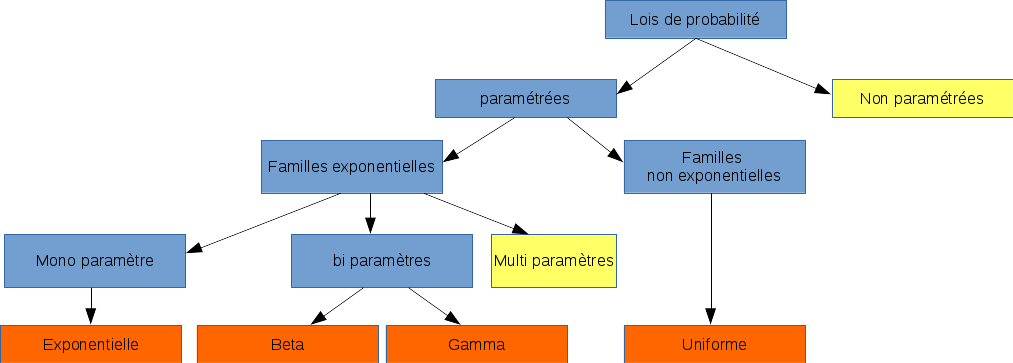
\includegraphics[width=\columnwidth]{taxonomieLoisStatistiques.png}
\caption{Taxonomie des lois statistiques utilisées.}
\label{fig:taxonomieLoisStatistiques}
\par}
\end{figure}

Pour soumettre les algorithmes à des données de situations réelle,
notre choix se porte sur la récupération (téléchargement) d'archives
existantes de listes de temps :
\lp{Dire ce que c'est}
\begin{itemize}
	\item PWA
\end{itemize}


\subsection{Génération des listes de temps synthétiques}\label{ssec:instancesGenerationListesTempsSynthetiques}
Les listes synthétiques sont créées de toutes pièces en suivant des lois statistiques et de distributions particulières. Sont présentées ici les lois EXPONENTIELLE, GAMMA, BETA et les 2 méthodes utilisées par \dcs UNIFORME et NON-UNIFORME.

\bigskip
\paragraph{Loi Exponentielle} 
ou loi de durée de vie, sans vieillissement (figure \ref{fig:LoiStatistiquesExponentielle}).
Soit $X$ une variable aléatoire définie dans $[0, \infty[$. $X$ suit une loi exponentielle de paramètre $\lambda$ si elle a pour densité :


  \begin{center}
  $[X=t] = \left\{
    \begin{array}{ll}
        \lambda e^{-\lambda t}  & \mbox{si } t \geq 0  \\
        0 & \mbox{sinon}
    \end{array}
	\right.$
  \label{definitionLoiExponentielleDensite}
  \end{center}

L’espérance et la variance sont fonctions de $\lambda$ et sont égales a :

\begin{align*}
	\E(X) &= \frac{1}{\lambda} \\
	\V(X) &= \frac{1}{\lambda ^2}
\end{align*} 


%--------------------------------------------------------
% Figure loi de statistique Exponentielle (flotante)
%--------------------------------------------------------
\begin{figure}
{\centering
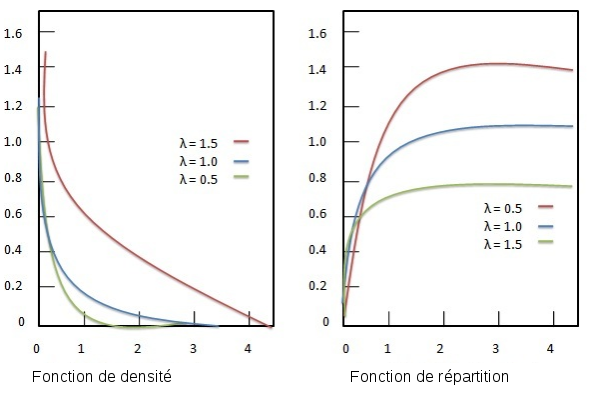
\includegraphics[width=\columnwidth]{loiStatExponentielle.png}
\caption{Loi statistique exponentielle.}
\label{fig:LoiStatistiquesExponentielle}
\par}
\end{figure}

\paragraph{Gamma}
ou modélisation de phénomènes qui se déroulent au cours du temps (figure \ref{fig:LoiStatistiquesGamma}). 
La loi de statistique Gamma est une loi de la famille des lois Exponentielles à 2 paramètres 
  et se définit sur $[0, \infty]$.
Si $Y_1, Y_2, \ldots, Y_n$ sont des variables I.I.D. 
  de loi exponentielle de paramètre $\lambda$ alors $X=\sum_{ i= 1}^{\alpha} X_i$  
  suit une loi Gamma $\Gamma(\alpha, \beta)$ avec 
    $alpha$ le paramètre de forme et 
    $\beta$ ($=\lambda$) le paramètre d'échelle. 
  
si X suit une loi $\Gamma(\alpha, \beta)$ alors la densité est de la forme :

  \begin{center}
  $[X=t] = \left\{
    \begin{array}{ll}
    	\frac{\beta^{\alpha} t^{\alpha-1} e^{-\beta t}}{\Gamma(\alpha)}  & 
    	\mbox{si } t \geq 0  \\
        0 & 
        \mbox{sinon}
    \end{array}
	\right.$
  \label{definitionLoiGammaDensite}
  \end{center}
   
Les paramètres $\alpha$ et $\beta$ peuvent être définis aussi ainsi :

   
\begin{align*}
   k 		& \textnormal{ tel que } \alpha = k  \textnormal{ et} \\
   \theta 	& \textnormal{ tel que } \beta  = \frac{1}{\theta}
\end{align*}

L’espérance et la variance sont fonctions de $k$ $\theta$ et sont égales a :

\begin{align*}
	\E(X) &= k \theta \\
	\V(X) &= k \theta ^2
\end{align*}

%--------------------------------------------------------
% Figure loi de statistique Gamma (flotante)
%--------------------------------------------------------
\begin{figure}
{\centering
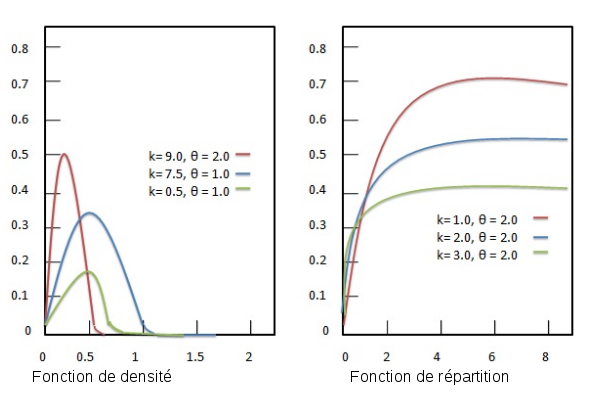
\includegraphics[width=\columnwidth]{loiStatGamma.png}
\caption{Loi statistique Gamma.}
\label{fig:LoiStatistiquesGamma}
\par}
\end{figure}

\paragraph{Beta} (figure \ref{fig:LoiStatistiquesBeta})
La loi Beta a été développée par Thomas Bayes (1702 - 1761) pour répondre à son propre problème 
  de succès/échecs dont la proportion de succès possible est inconnue \cite{bayes1991essay}. Cette proportion inconnue, qui est la variable aléatoire représentée par une loi beta, est déduite par tirages successifs avec remise. 
La loi de statistique Beta est une loi de la famille des lois Exponentielles à 2 paramètres et se définit 
  sur $[0, \infty]$. 
 
% texte traduit de Bayes
%  étant donné un certain nombre de fois où un événement inconnu s'est produit et a échoué : il faut que %la probabilité qu'il se produise lors d'un seul essai se situe quelque part entre deux degrés de %probabilité que l'on peut nommer. 

Si la variable aléatoire X suit une loi Beta de paramètres $\alpha$ et $\beta$ alors la loi de densité est de la forme :
  \begin{center}
  $[X=t] = \left\{
    \begin{array}{ll}
    \frac{\Gamma(\alpha + \beta) t^{\alpha-1} (1-t)^{\beta-1}}{\Gamma(\alpha) \Gamma(\beta)}
    & 
   	\mbox{si } t \in [0,1]  \\
        0 & 
        \mbox{sinon}
    \end{array}
	\right.$
  \label{definitionLoiBetaDensite}
  \end{center}

Beta est intéressante dans l'analyse de proportions d’événements de type succès/échec ou
(moyennant un changement d'échelle) dans la modélisation du temps avant la fin d'une tâche.

L’espérance et la variance sont fonctions de $\alpha$ $\beta$ et sont égales a :

\begin{align*}
	\E(X) &= \frac{\alpha}{\alpha + \beta} \\
	\V(X) &= \frac{\alpha \beta}{(\alpha + \beta)^2 (\alpha + \beta + 1)} 
\end{align*}

%--------------------------------------------------------
% Figure loi de statistique Beta(flotante)
%--------------------------------------------------------
\begin{figure}
{\centering
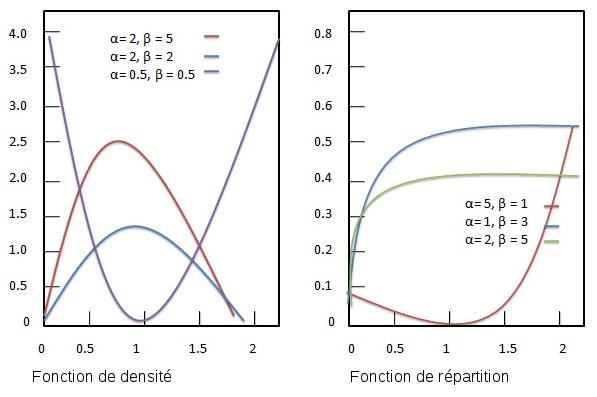
\includegraphics[width=\columnwidth]{loiStatBeta.png}
\caption{Loi statistique Beta.}
\label{fig:LoiStatistiquesBeta}
\par}
\end{figure}



\paragraph{Uniforme} Cette loi statistique, utilisée pas \dcs est non exponentielle. 
Une loi UNIFORME sur $[a, b]$ est une loi de probabilité $P$ dont la fonction de densité et 
  constante sur $[a, b]$. i.e. les nombres générés sont uniformément répartis dans l'intervalle $[a, b]$

\begin{center}
$[X] = \frac{1}{b-a}$
\end{center}

\paragraph{Non-uniforme} Ce type de génération de liste de temps est utilisé dans le protocole expérimental de \cite{frangioni2004multi} et est repris par \dcs \cite{della2020longest} pour éprouver SLACK.
Une liste de nombres aléatoires générée via une règle NON-UNIFORME de paramètres $a$ et $b$ 
  est l'union de 2 listes générées via une loi uniforme comme suit :

\begin{align*}
	98 \%  &= \textnormal{loi uniforme } [0.9(b-a), b] \\
	2\%    &= \textnormal{loi uniforme } [a, 0.2(b-a)] 
\end{align*}

\jb{En vrai, ça devrait être $[a + 0.9 (b-a), b]$ et $[a, a + 0.2 (b-a)]$}

\begin{example}
Pour la génération d'une liste suivant la règle non-uniforme [1, 100], 

\begin{align*}
	98 \%  &\textnormal{ est uniformément répartis sur } [89.1~~ 100] \\
	2\%    &\textnormal{ est uniformément répartis sur } [1   ~~ 19.8] 
\end{align*}

\end{example}
\lp{}
 
\subsection{Récupération de listes de temps réelles}\label{ssec:instancesGenerationListesTempsReelles}

\paragraph{PWA} Parallel Workload Archive. L'idée est de collecter des données de vrais systèmes et de 
  supposer que les futurs workload seront similaires \cite{feitelson2014experience}.

   
PWA est un dépôt de fichiers journaux de temps disponible à 
  l'URL :
  
\url{https://www.cs.huji.ac.il/labs/parallel/workload/}

Ces archives proviennent de l'enregistrement direct des événements qui se produisent sur les systèmes informatiques et ont l'avantage de représenter un panel de besoins réels. 
Mais elles peuvent comporter certains inconvénients :
\lp{attention majuscules/minuscules dans la liste}
\begin{itemize}

	\item Le nombre de jobs $n$ n'est pas maîtrisé, et ne représente qu'une 
	vingtaine de fichiers, donc un nombre limité de tests et comparaisons empiriques à effectuer.
	
	\item Ces archives ne sont pas forcément complètes et certaines informations importantes peuvent manquer.
	
	\item incohérence de données. Certaines informations ne passent pas le con\-trôle de
	contraintes d'intégrités.
	
	\item Données erronées. Des données peuvent être fausses. e.g dues au dépassement d'adressage de nombres.
	
	\item modification d'environnement. Le problème inhérent aux machines 
	est leur hétérogénéité qui change avec le temps.
	
	\item Comportement non représentatif. L'aspect humain entre aussi en ligne de compte.
	
	\item Effet "END". Les jobs sont consignés une fois terminés. 
	Entre une tâche extrêmement courte et une tâche longue le temps 
	d'enregistrement est le même. Cela peut provoquer un décalage 
	entre la fin du journal et le temps calculé.
	
	\item Les temps d'arrêts ne sont pas consignés. 
	  
\end{itemize}

\subsection{Instance et maîtrise de la solution optimale}
\label{ssec:instancesMaitriseSolutionOptimale}

Pour comparer les résultats obtenus, il est nécessaire d'avoir un référent par rapport au Makespan. 
Il n'est pas possible d'obtenir le ratio d'approximation de l'algorithme A ($\Gamma(A)=\frac{C_m^A(J)}{C_m^\star(J)}$) car l'optimal n'est pas connu et c'est précisément ce que l'on cherche. 
La seule donnée connue est la borne minimale de la liste de tailles de jobs.
Or cette borne ($\text{borne}_{min} = \max \{ \max_i\{p_i\}, \frac{1}{m} \sum_{i=1}^{n} p_i \}$) n'est pas forcément l'optimal et le rapport $\frac{Optimal}{\text{borne}_{min}}$ varie.

\bigskip
% Exemple
% ---------------------

\begin{figure}
{\centering
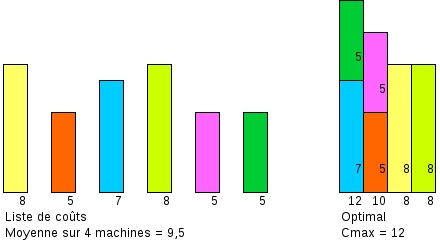
\includegraphics[width=\columnwidth]{MoyenneVsOptimal.jpg}
\caption{Liste de coût de départ, moyenne des tailles des jobs pour 4 machines, et makespan optimal.}
\label{ex:borneMinVSOptimalListeDepart}
\par}
\end{figure}

\begin{example}
Soit $P=\{8, 5, 7, 8, 5, 5\}$, l'ensemble des $p_i$ à appliquer sur 4 machines parallèles identiques.
La borne minimale est:

$$\text{borne}_{min} = \max \left\{ \max_i\{p_i\}, \frac{1}{m} \sum_{i=1}^{n} p_i \right\} = 9.5$$

L'optimal $C_4^\star(J) = 12$ (figure \ref{ex:borneMinVSOptimalListeDepart}).
\end{example}

Cette borne minimale est égale à l'optimal uniquement si toutes les char\-ges des machines sont identiques.
À partir d'une liste de coûts (synthétique ou naturelle) il est donc possible d'obtenir une instance dont l'optimal est connu \cite{benoit2021update}. Cette opération nécessite la transformation de la liste de coût de départ pour un
  nombre de machines défini (figure \ref{ex:maitriseOptimal}).
\begin{itemize}
	\item Soit une liste de $n$ jobs et l'ensemble des $p_i$ à appliquer sur $m$ machines parallèles identiques.
	\item Ordonnancement : chaque job est affecté à la machine la moins chargée à ce moment là.
	\item Tri : tri des machines par ordre décroissant des charges.
	\item Complétion : la machine la plus chargée (la première) représente le MakeSpan. La charge des $m-1$ machines restantes est complétée
              \lp{Avec des tâches fictives} pour obtenir le même temps
              d'exécution que la machine la plus chargée.
  \jb{Attention à écrire makespan toujours de la même manière tout au long du rapport}
	\item toutes les machines ont le même temps d'exécution. L'optimal, est dans ce cas égal à la 
	      moyenne des temps par machine. 
	      La nouvelle liste de coûts contient désormais $n + m-1$ éléments.
\end{itemize}

\bigskip 
Il convient de distinguer la liste de coût Native obtenue 
  soit par génération, 
  soit par récupération, 
  dont seule la borne minimale est connue, 
  et sa transformée, complétée avec $m-1$ temps de jobs, nommée M1 (qui est une instance), 
  dont l'optimal est connu.
Tous les tests sont effectués sur les instances M1, 
  et sur le nombre réel de tâches ($n + (m-1)$).

\begin{figure}
{\centering
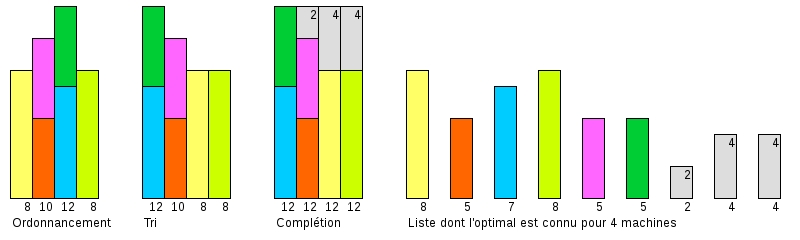
\includegraphics[width=\columnwidth]{maitriseOptimal.jpg}
\caption{transformation d'une liste pour obtenir l'optimal.}
\label{ex:maitriseOptimal}
\par}
\end{figure}

\subsection{Indicateurs statistiques et caratéristiques}\label{ssec:instancesIndicateursStatistiquesCaratéristiques}

\jb{A-t-on vraiment besoin de cette section vu qu'on ne donne pas ces indicateurs pour les listes utilisées par la suite?}

Afin de caractériser une liste de coût, plusieurs indicateurs statistiques sont calculés à la génération, ou à la récupération de celle-ci.

\begin{itemize}
	\item La moyenne de la charge par machine;
	\item La moyenne des éléments de $P$;
	\item La moyenne géométrique des éléments de $P$;
	\item La médiane de l'ensemble $P$;
	\item Le plus petit élément de $P$;
	\item Le plus grand élément de $P$;
	\item L'écart type des valeurs de $P$;
	\item La variance des valeurs de $P$.
\end{itemize}

Ces divers indicateurs peuvent donner une appréciation quant à 
  l'hétérogénéité d'une liste de temps, ou d'une instance.


\bigskip
Nous venons de voir comment les listes de temps sont générées et utilisées. 
Elles peuvent être créées via la production de nombres pseudo-aléatoires selon un nombre 
  défini de jobs et une distribution statistique choisie, 
  ou récupérées d'une archive de fichiers journaux de tâches relatifs à de réelles 
  activités de production.
De ces listes, peuvent être calculées des instances (M1) dont l'optimal est connu, 
  ce qui va permettre une estimation de l'efficacité des algorithmes.
Et enfin, plusieurs indicateurs statistiques caractérisant chaque instance les accompagnent.

Nous abordons maintenant la notion de ``campagnes'' de tests où les instances sont soumises à des heuristiques.  

% =======================================================
% 4 CAMPAGNES
% =======================================================
\section{Campagnes} \label{sec:Campagnes}

Chaque tests se déroule en ``campagne''. 

%--------------------------------------------------------
% plan
%--------------------------------------------------------
Ce chapitre aborde l’environnement de tests, le choix des heuristiques implémentés et le déroulement d'une campagne. Est expliqué, pour finir, comment les Makespan sont comparés entre eux.

\subsection{Environnement de tests} \label{ssec:campagnesEnvironnementDeTests}

L'environnement de tests est développé 
  en PYTHON pour la partie applicative 
  (génération des listes de temps, calcul de l'instance M1, algorithmes) et 
  en R pour la partie analyse et graphes. 
Des informations sur la plate-forme sont disponibles en annexe.

Toutes les campagnes ont été effectuées sur un portable 
  doté de 4 Go de ram et 
  équipé d'un processeur Intel core I3 4330u cadencé à 1900 MHz.


\subsection{Choix des heuristiques} \label{campagneChoisHeuristiques}

Pour reproduire l'expérience de \dcs et comparer les résultats, les mêmes heuristiques sont implémentées à l'environnement de test. Soit :
\begin{itemize}
	\item LPT rule
	\item SLACK
	\item LDM
	\item COMBINE
\end{itemize}

Ceci a aussi l'avantage d'expérimenter 4 pistes différentes étudiées 
  pour résoudre le problème \problemGrahamP :
\begin{itemize}
	\item LS (list-Scheduling) avec LPT rule; 
	\item Bin-Packing avec COMBINE; 
	\item Strategie gloutonne avec SLACK; 
	\item Partitionnement de nombres avec LDM.  
\end{itemize}

COMBINE repose sur deux autres heuristiques qui sont aussi implémentées : FFD et MULTIFIT.



\subsection{Déroulement d'une campagne} \label{ssec:campagnesDeroullementDUneCampagne}
L'objectif est de reproduire le protocole expérimental de \dcs et aussi de l'élargir 
  à d'autres types d'instances et de possibilités de comparaisons.
En plus des possibilités de tests sur des instances de 10, 50, 100, 500 et 1000 jobs à planifier 
  sur 5, 10 et 25 machines \cite{della2020longest}, 
  chaque campagne peut faire varier $n$ de 1 en 1 avec 
  un nombre de départ, et un nombre d'arrivée, 
  ou suivant une liste. 
Il en est de même pour le nombre de machines $m$. 
Les deux valeurs peuvent aussi évoluer conjointement.

%--------------------------------------------------------
% Figure déroulé d'une campagne (flotante)
%--------------------------------------------------------
\begin{figure}
{\centering
%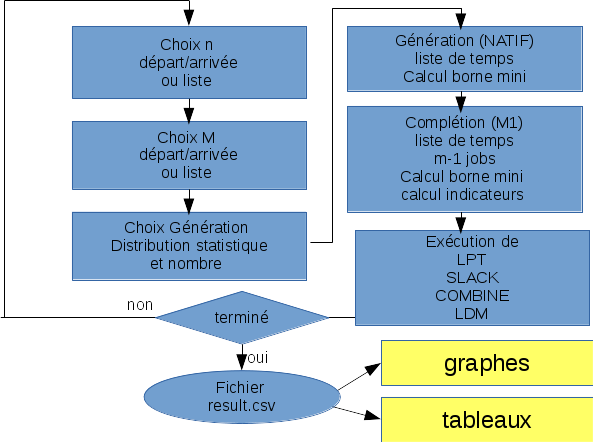
\includegraphics[width=\columnwidth]{derouleCampagne.png} : trop grand sinon!
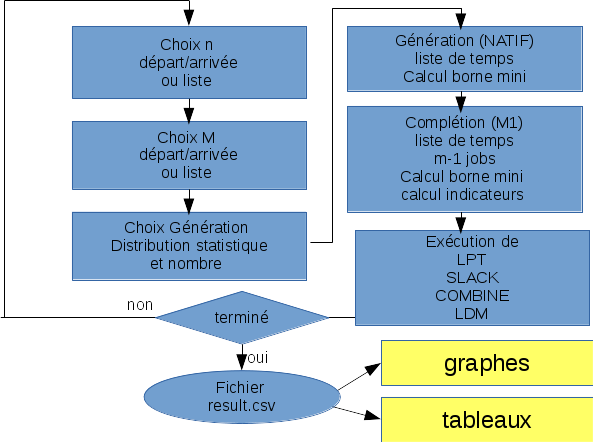
\includegraphics[height=50mm]{derouleCampagne.png}
\caption{Déroulement d'une campagne.}
\label{fig:deroulementDUneCampagne}
\par}
\end{figure}

Une campagne boucle sur le nombre de machines choisies, le nombre de jobs à créer pour les listes de temps, par nombre et type de loi statistiques. Pour chaque triplet \{$m$, $n$, liste de temps\} une instance native et M1 sont créées, et les algorithmes LPT, SLACK LDM et COMBINE sont soumis (figure \ref{fig:deroulementDUneCampagne}).

Les 4 algorithmes sont donc soumis à chaque itération, aux mêmes instances i.e aux mêmes valeurs. 

%--------------------------------------------------------
% Figure Contenu fichier RESULT.CSV (flotante)
%--------------------------------------------------------
\begin{figure}
{\centering
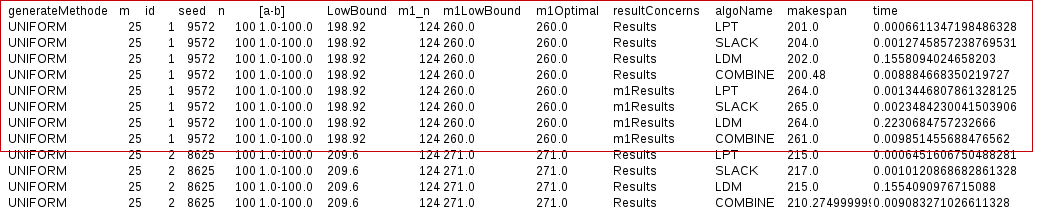
\includegraphics[width=\columnwidth]{contenuResultCSV.png}
\caption{Contenu du fichier result.csv.}
\label{fig:contenuResultCSV}
\par}
\end{figure}

8 lignes résultat sont générées et sont intégrées dans un fichier global ``result.csv'' une fois les boucles de la campagne terminées pour comparaison des résultats (figure \ref{fig:contenuResultCSV}). La structure se décompose ainsi :
\begin{itemize}
	\item generateMethode : est la méthode qui est utilisée pour générer la liste de temps. 
	\item m : est le nombre de machines identiques pur les instances Native et M1 
	\item id : est l'id du triplet \{$m$, $n$, numéro de liste de temps\}. 
			Sert aux regroupements et comparaisons des algorithmes pour une même instance.
	\item seed : est a graine résultante du moteur de génération de nombre pseudo-aléatoires 
			utilisé pour la création de la liste de temps. Peut servir pour recréer à 
			l'identique une instance. 
	\item n : Nombre de jobs servant à créer une liste de temps native. 
	\item $[a-b]$ : Paramètres a et b pour les listes de temps UNIFORME et NON-UNIFORME. 
			cette information est utilisée pour recréer le protocole expérimental 
			de Della Croce et Scatamacchia.
	\item LowBound : Borne inférieure de l'instance native.
	\item m1\_n : Nouveau nombre de jobs de l'instance M1 après complétion et calcul 
			de l'optimal.
	\item m1LowBound : Borne inférieure de l'instance M1.
	\item m1Optimal : Optimal calculé sur l'instance M1.
	\item resultConcerns : indique si le Makespan calculé concerne l'instance native ou M1.
	\item algoName : Nom de l'algorithme soumis.
	\item makespan : Makespan trouvé par l'algorithme soumis.
	\item time : Temps qu'il a été nécessaire pour calculer le makespan 
			par l’algorithme soumis. 
\end{itemize}

\subsection{Comparaison Makespan et normalisation}
 \label{ssec:campagnesComparaisonMakespanNormalisation}

Comparer les Makespans obtenus n'est pas significatif. Les valeurs obtenues sont fonction des valeurs de temps des instances.

Il est donc nécessaire de normaliser le résultat pour permettre des comparaisons. 3 pistes sont explorées :
\begin{itemize}

  \item $\frac{Makespan}{borne~inférieure}$ : seule piste possible de normalisation 
  des instances natives, car seule, leur borne inférieure sont connues. 
  C'est la normalisation qui est utilisée pour comparer les algorithmes sur 
  des instances natives.
  
  \item Makespan - Optimal : ou Makespan absolu \cite{benoit2021update}. 
  Permet de retirer du résultat l'optimal connu de l'instance M1.
  Cette valeur tend vers $0$ lorsque le résultat converge vers l'optimal, 
  mais ne permet pas une comparaison avec 
  le ratio d'approximation $\Gamma(A)=\frac{C_m^A(J)}{C_m^\star(J)}$.

  \item $\frac{Makespan}{Optimal}$ : ou Makespan relatif \cite{benoit2021update}.
  Permet d'obtenir le rapport entre le Makespan calculé et l'optimal de l'instance M1.
  Cette valeur tend vers $1$ lorsque le résultat converge vers l'optimal, 
  Cette normalisation permet aussi une comparaison avec  
  le ratio d'approximation $\Gamma(A)=\frac{C_m^A(J)}{C_m^\star(J)}$. 
  Cette normalisation est donc utilisée pour comparer les résultats obtenus sur les instances 
  M1.
\end{itemize}


% =======================================================
% 5 RESULTATS
% =======================================================
\section{Résultats} \label{sec:resultats}

\lp{Dans la suite on utilise que des instances M1 ?}

\subsection{Protocole expérimental de Della Croce et Scatamacchia}
\label{ssec:resultatsPrtocoleExperimentalDellaCroceScatamacchia}
 
Pour comparer SLACk aux autres heuristiques, LPT, LDM et COMBINE, Della Croce et Scatamacchia 
 utilisent 10 instances UNIFORMES et NON-UNIFORMES d'intervalle [a, b] de [1, 100], [1, 1000] et [1, 10000], pour un nombre de machines de 5 et un nombre de jobs de 10, 50, 100, 500 et 1000, et sur un nombre de machines de 10 et 25 pour un nombre de jobs de 50, 100, 500 et 1000.
soit un total de : 

pour chaque intervalle [a, b] = [1, 100], [1, 1000], [1, 10000] et
  chaque classe UNIFORM et NON-UNIFORM 
\begin{itemize}
\item 10 instances $\cdot$ 5 couples $\{m=5,n\}$: \\ $\{5,10\},\{5,50\},\{5,100\},\{5,500\},\{5,1000\}$
\item 10 instances $\cdot$ 4 couples $\{m=10, n\}$: \\ $\{10,50\},\{10,100\},\{10,500\},\{10,1000\}$
\item 10 instances $\cdot$ 4 couples $\{m=25,n\}$: \\ $\{25,50\},\{25,100\},\{25,500\},\{25,1000\}$
\end{itemize}  

780 instances.

\lp{Pour le tableau iL faut expliquer W/E/L}

%--------------------------------------------------------
% Figure resultat obtenu par DCS (non flottant
%--------------------------------------------------------
\begin{figure}
{\centering
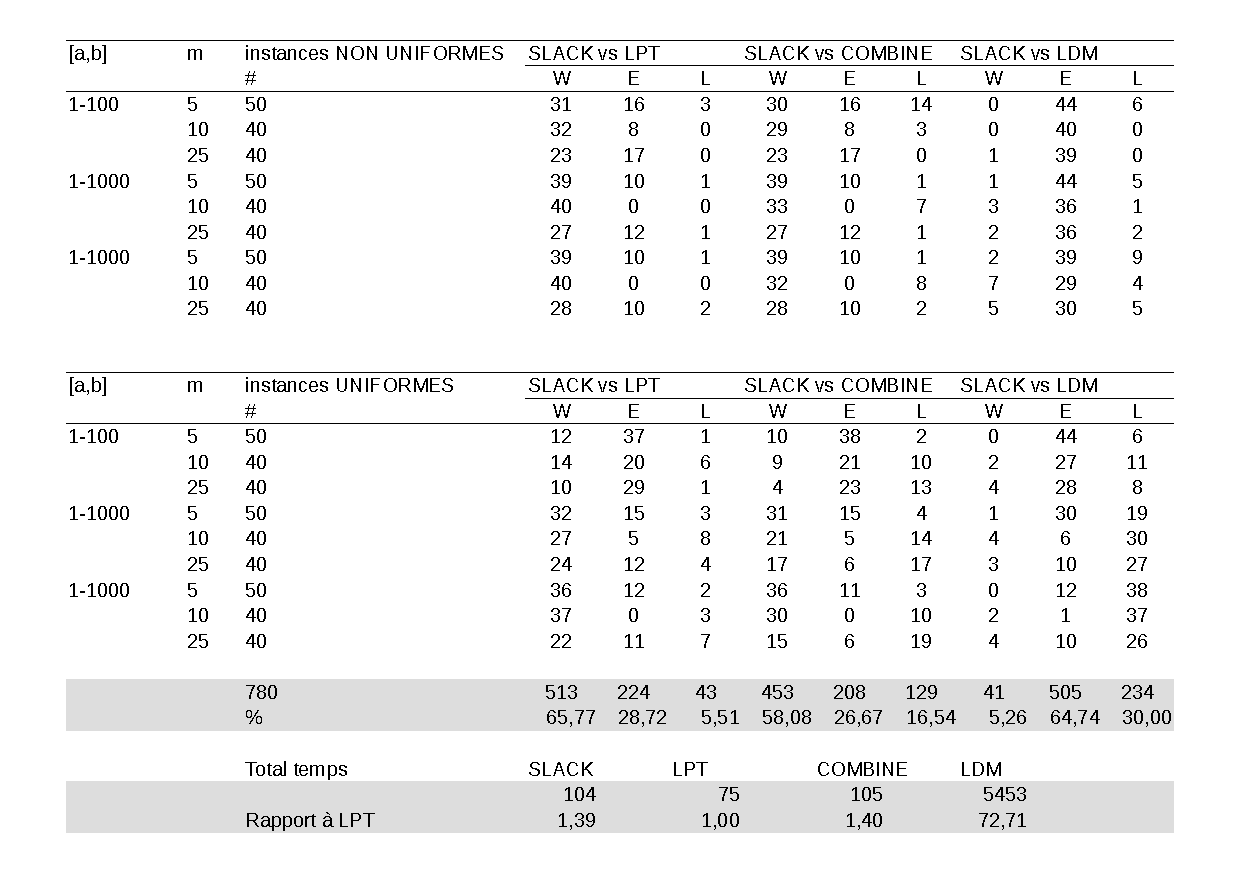
\includegraphics[width=\columnwidth]{1_Resultat_De_DCS.pdf}
%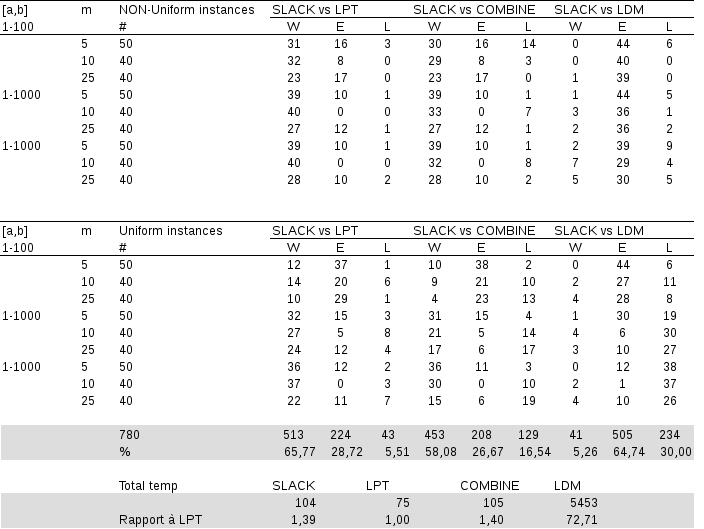
\includegraphics[height=100mm]{1_Resultat_De_DCS.png}
\caption{Résultat obtenu par Della Croce et Scatamacchia.}
\label{fig:resultatDellaCroceScatamacchia}
\par}
\end{figure}

La figure \ref{fig:resultatDellaCroceScatamacchia} représente le résultat obtenu 
  dans \cite{della2020longest}. 
Les auteurs annoncent une amélioration significative de LPT avec SLACK, 
  car celui-ci est meilleur à 65.8\% des cas contre LPT, suivant les 780 instances 
  de référence de la littérature \cite{della2020longest}. De ce fait, SLACK peut être vu comme une alternative précieuse à LPT.
  
  
\subsection{SLACK sur des instances réelles}
\label{ssec:resultatsSLACKReel}

%--------------------------------------------------------
% Figure resultat obtenu par DCS (flottant)
%--------------------------------------------------------
\begin{figure}
{\centering
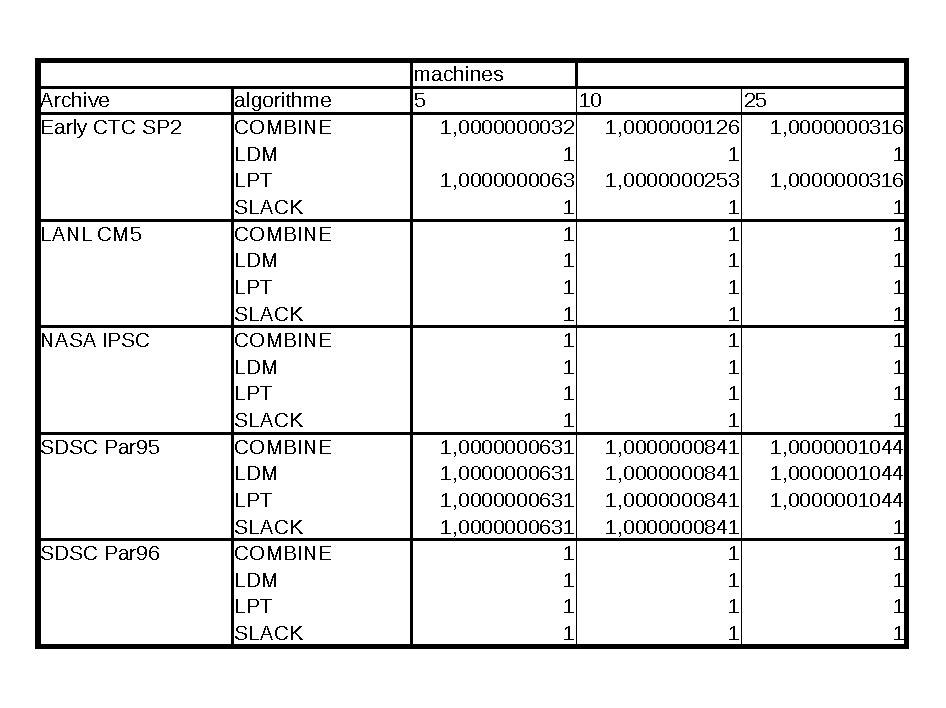
\includegraphics[width=\columnwidth]{2_Resultat_reel.pdf}
\caption{Résultat sur 5 archives PWA.}
\jb{Qu'est-ce que représentent ces nombres? Il faut le dire dans le titre}
\label{fig:resultat5PWA}
\par}
\end{figure}
 
 Les 4 algorithmes sont exécutés sur des listes de temps réelles, provenant de 5 PWA NASA IPSC, Early CTC SP2, LANL CM5, SDSC Par95 et SDSC Par96, qui contiennent respectivement 18066, 75895, 122058, 32128 et 53744 jobs. Ces 5 archives sont transformées en instances de 5, 10 et 25 machines, et le résultat est représenté en figure~\ref{fig:resultat5PWA}.
 
SLACK est efficace, mais de très peu. 
Les heuristiques, dans cet échantillons, sont plus souvent équivalentes.  
 
\subsection{Reproduction du protocole expérimental de Della Croce et Scatamacchia}
\label{ssec:resultatsReroductionPrtocoleExperimentalDellaCroceScatamacchia}
 
%--------------------------------------------------------
% Figure resultat obtenu par REPRODUCTION DU PROTOCOLE DE DCS
%--------------------------------------------------------
\begin{figure}
{\centering
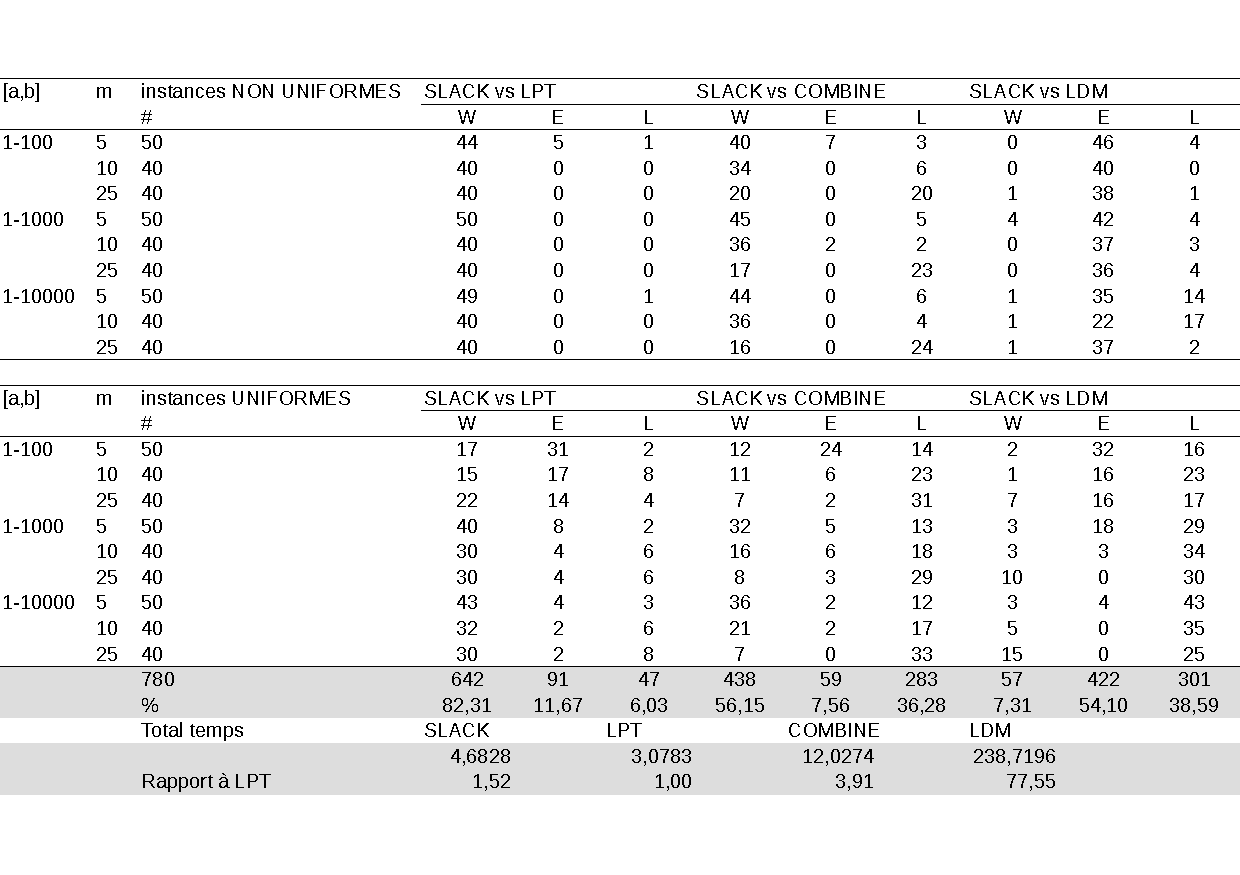
\includegraphics[width=\columnwidth]{3_Resultat_Reproduction_De_DCS.pdf}
\caption{Résultat obtenu par reproduction Della Croce et Scatamacchia.}
\label{fig:resultatReproductionDellaCroceScatamacchia}
\par}
\end{figure}

Le même protocole expérimental est exécuté. Le résultat est indiqué 
  figure~\ref{fig:resultatReproductionDellaCroceScatamacchia}.
Les résultats obtenus ne sont pas tout à fait identiques ou avoisinants. 
  
Côté temps, SLACK passe d'un rapport de 1.3 à un rapport de 1.5 par rapport à LPT. 
Mais c'est COMBINE qui a le plus de différence en passant d'un rapport de 1.40 
  à un rapport de 3.9 par rapport à LPT. 
Cela peut être du à l'implémentation des algorithmes et à la technologie utilisée. 

Coté Makespan, SLACK cumule plus de victoires contre LPT, en passant de 65.8\% à 82.3\% de ``WIN''.
Par contre, SLACK perd de son efficacité contre LDM et surtout contre COMBINE. COMBINE qui récupère 36.3\% de ``WIN'' contre SLACK, contre 16.5\% précédemment indiqué.


Peut-être que notre protocole est une singularité statistique. L'expérience est exécutée 50 fois, pour s'approcher le plus de la tendance la plus représentative.


%--------------------------------------------------------
% Figure resultat obtenu par REPRODUCTION DU PROTOCOLE DE DCS
%--------------------------------------------------------
\begin{figure}
{\centering
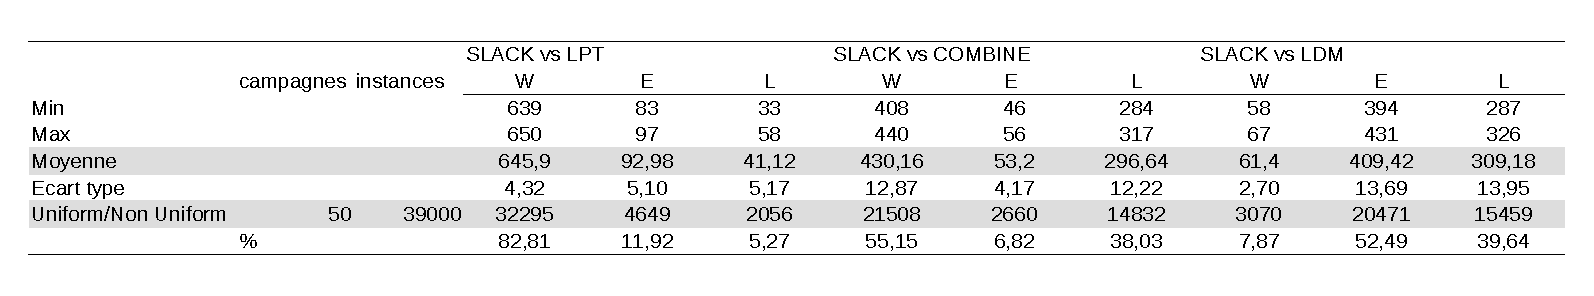
\includegraphics[width=\columnwidth]{4_Resultat_Reproduction50DCS.pdf}
\caption{Résultat obtenu avec 50 campagnes de tests type ``Della Croce et Scatamacchia''.}
\label{fig:resultatReproduction50DellaCroceScatamacchia}
\par}
\end{figure}

Le résultat est résumé en figure \ref{fig:resultatReproduction50DellaCroceScatamacchia}. 
La tendance des 50 campagnes corrèle le résultat obtenu précédemment et non pas 
  celui de Della Croce et Scatamacchia.

\subsection{Influence des distributions sur le comportement des heuristiques}
\label{ssec:resultatsInfluenceDesDistributionSurLeComportement}


Della Croce et Scatamacchia ne comparent les algorithmes que sur 2 familles de distributions : 
UNIFORME et NON-UNIFORME. Distributions générées avec 3 paramètres différents, le résultat est synthétisé avec des instances de 5, 10, 25 machines, et 10, 50, 100, 500, 1000 jobs. 
Les différences trouvées entre notre expérience et celle de Della Croce et Scatamacchia peuvent 
être dues à une variété trop grande de paramètres , résumés en un seul résultat.

\bigskip
Pour vérifier si la distribution statistique utilisée pour générer les listes de temps 
  a une influence sur le résultat, 
  nous reprenons la même expérience, avec 2 autres familles de distributions : 
  Gamma et Beta de paramètres $\alpha = 1$ et $\beta = 1$,
  sur des instances de 5, 10, 50, 100, 500, 1000 jobs, 
  à ordonnancer sur 5, 10, 25 machines,
  sur 10 campagnes.

Le résultat est donné figure \ref{fig:resultatReproduction10GammaBeta}.
SLACK descend à 68.7\% contre LPT, 
n'est plus qu'à 43,4\% contre COMBINE et
à 13.5\% contre LDM

\bigskip
Le type d'instance a une influence sur le comportement des algorithmes, notamment sur l'efficacité de SLACK.
   
%--------------------------------------------------------
% Figure resultat obtenu par 10 cmpagnes type DCS mais en Gamma/Beta
%--------------------------------------------------------
\begin{figure}
{\centering
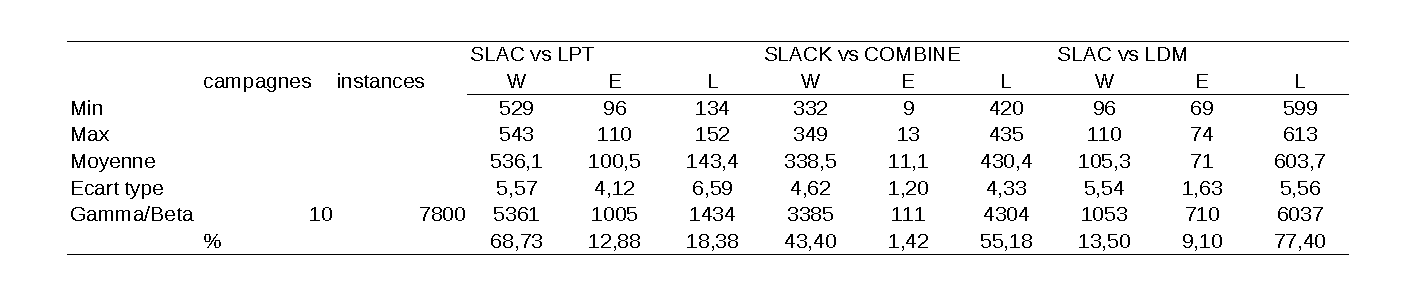
\includegraphics[width=\columnwidth]{5_Resultat_Reproduction10GammaBeta.pdf}
\caption{Résultat obtenu avec 10 campagnes de tests avec des distributions Gamma et Beta.}
\label{fig:resultatReproduction10GammaBeta}
\par}
\end{figure}

\bigskip
Nous reprenons la même expérience, avec les 2 familles de distributions 
  Gamma et Beta de paramètres $\alpha = 1$ et $\beta = 1$,
  des instances uniquement de 1000 jobs à ordonnancer sur 5, 10 et 25 machines,
  sur 10 campagnes.
\lp{Dire pourquoi tu fais ça}
%--------------------------------------------------------
% Figure resultat obtenu par 10 cmpagnes type DCS mais en Gamma/Beta et 1000 jobs
%--------------------------------------------------------
\begin{figure}
{\centering
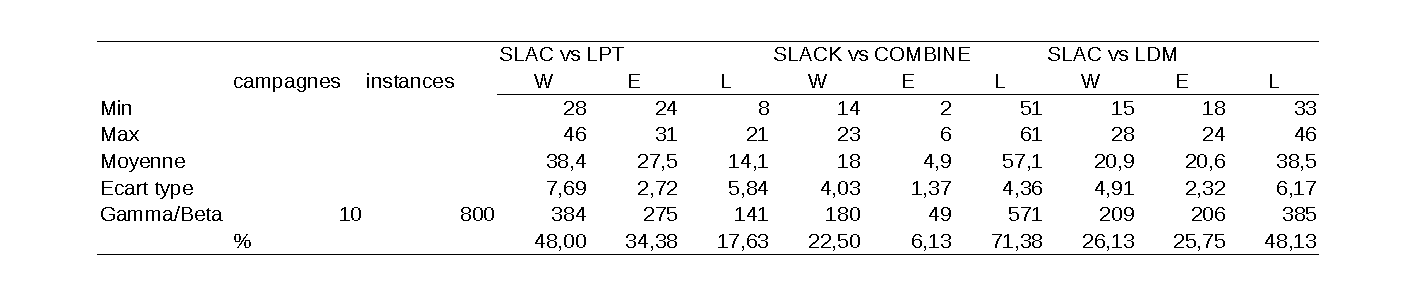
\includegraphics[width=\columnwidth]{6_Resultat_Reproduction10GammaBeta1000.pdf}
\caption{Résultat obtenu avec 10 campagnes de tests avec des distributions Gamma et Beta sur des instances de 1000 jobs.}
\label{fig:resultatReproduction10GammaBeta1000}
\par}
\end{figure}

Le résultat en figure \ref{fig:resultatReproduction10GammaBeta1000} indique que 
  SLACK ne domine plus LPT avec 48\% de ``WIN'' et
  laisse l'efficacité à COMBINE et LDM avec respectivement 22,5\% et 26,1\%.



\bigskip
Nous retirons la loi de distribution beta dans la génération des listes de temps.
Donc 1 familles de distributions Gamma, 
  des instances uniquement de 1000 jobs à ordonnancer sur 5, 10 et 25 machines,
  sur 10 campagnes.
\lp{Dire pourquoi tu fais ça}
%--------------------------------------------------------
% Figure resultat obtenu par 10 cmpagnes type DCS mais en Gamma et 1000 jobs
%--------------------------------------------------------
\begin{figure}
{\centering
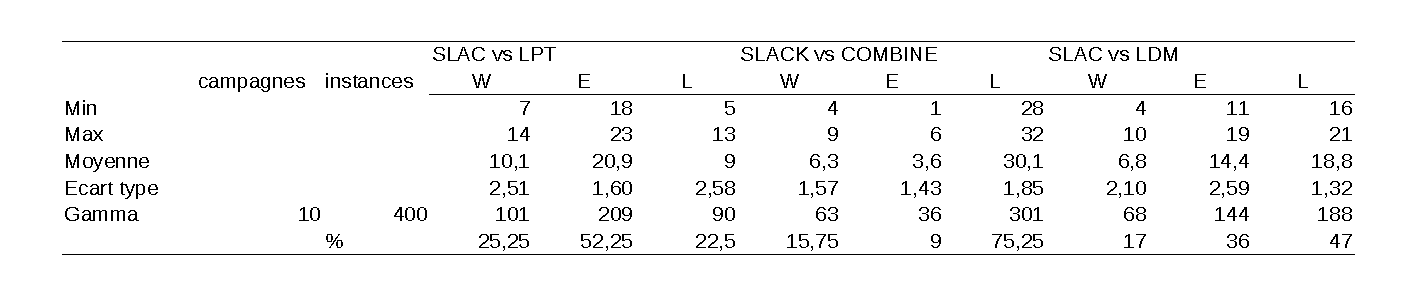
\includegraphics[width=\columnwidth]{7_Resultat_Reproduction10Gamma1000.pdf}
\caption{Résultat obtenu avec 10 campagnes de tests avec une distribution Gamma sur des instances de 1000 jobs.}
\label{fig:resultatReproduction10Gamma1000}
\par}
\end{figure}

SLACK n'est plus qu'à 25\% contre LPT, 15\% contre COMBINE et 17\% contre LDM (figure \ref{fig:resultatReproduction10Gamma1000}).

\jb{Il manque une tentative d'explication sur pourquoi SLACK est moins bon sur des distributions gamma ou beta}

\subsection{Cartographie des heuristiques}
\label{ssec:resultatsCartographie}

Della Croce et Scatamacchia utilisent des instances de 10, 50, 100, 500 et 1000 jobs à ordonnancer sur 5, 10 et 25 machines. 
Ce qui représente 13 points de tests 
  (les instances 
  $\{10~jobs,10~machines\}$ et 
  $\{10~jobs,25~machines\}$ n'existent pas car $m\geq n$).
En faisant évoluer $n$ de 10 à 1000 et $m$ de 5 à 50, 
  et en consignant l'algorithme (entre LPT et SLACK) qui donne 
  le Makespan relatif le plus bas, nous obtenons le graphe en figure \ref{fig:resultatComparaisonLPTSLACK}.
Les points rouges représentent les 13 points de test en question.

%--------------------------------------------------------
% Figure resultat comparaison de LPT et SLACK sur n et m
%--------------------------------------------------------
\begin{figure}
\centering
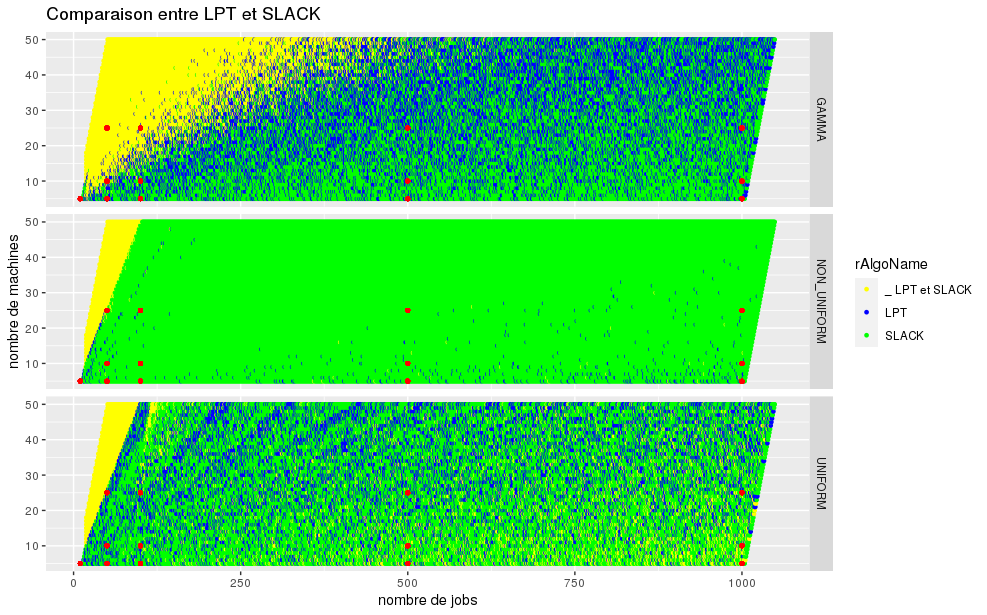
\includegraphics[width=\columnwidth]{8_comparaison_LPT_SLACK_2D.png}
\caption{comparaison LPT et SLACK sur 3 distributions avec $10\leq n \leq 1000$ et $5\leq m \leq 50$}
\label{fig:resultatComparaisonLPTSLACK}
\end{figure}

\lp{Parler de la partie jaune optimale ? D'ailleurs on peut signaler
  qu'il n'y a pas de jaune..}

En distribution UNIFORME, SLACK domine largement avec 
  un petit nombre de machines. Mais en montant en $m$, LPT devient un peu 
  plus présent.
En distribution NON-UNIFORME, SLACK est vraiment plus efficace que
LPT.\lp{Tu as une idée de la raison ?}
Par contre, en distribution Gamma, LPT devient vraiment plus efficace.

Il est à remarquer que les points rouges du protocole expérimental de 
  Della Croce et Scatamacchia sont placés principalement à des coordonnées
  où SLACK domine (dans les instances à distribution UNIFORME et NON-UNIFORME).

%--------------------------------------------------------
% Figure resultat comparaison de tous les algorithmes 
%--------------------------------------------------------
\begin{figure}
{\centering
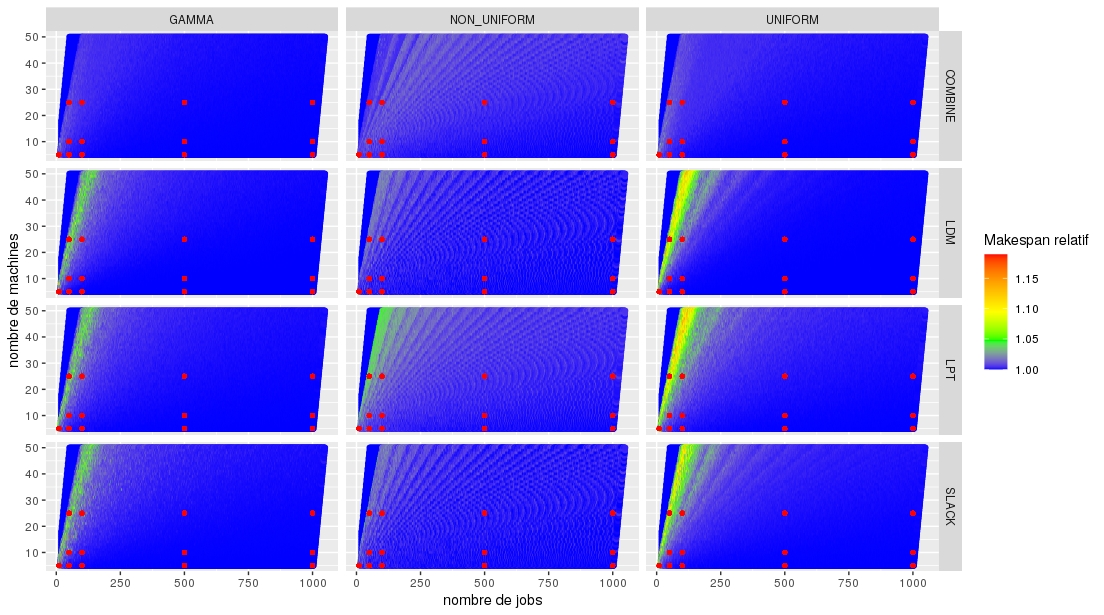
\includegraphics[width=\columnwidth]{9_resultatComparaisonAlgoDistributions.jpeg}
\caption{comparaison LPT, SLACK, COMBINE, LDM par algorithme, et par distribution avec $10\leq n \leq 1000$ et $5\leq m \leq 50$}
\label{fig:resultatComparaisonAlgoDistributions}
\par}
\end{figure}

La figure \ref{fig:resultatComparaisonAlgoDistributions} \lp{verbe ?} une infime partie 
  du comportement de chaque algorithme par famille de distribution 
  (Gamma, NON-UNIFORME et UNIFORME) 
  pour des instances, dont le nombre de machines est compris entre 5 et 50, 
  et le nombre de jobs varie de 10 à 1000. 

Il est à noter plusieurs phénomènes remarquables :
\begin{itemize}
	\item En distribution Gamma, les algorithmes se stabilisent 
	assez rapidement plus le nombre de jobs $n$ est élevé.
	
	Le Makespan relatif dessine une bande oblique de ``pires cas'' 
	qui suit la ligne $n = 2m$ , pour rapidement converger vers 1 
	lorsque $n$ augmente. 
	Cette bande est de plus en plus épaisse avec un nombre 
	élevé $m$ de machines.
	 
	\item En distribution UNIFORME, SLACK converge moins rapidement que 
	LPT et LDM. Mais de façon générale, plus le nombre de machines $m$ 
	est élevé, plus la convergence vers 1 du Makespan relatif nécessite 
	un nombre élevé $n$ de jobs.
	
	Le Makespan relatif dessine des vagues obliques de ``pires cas'' 
	qui débutent suivant la ligne $n = 2m$ , pour s'estomper petit à petit 
	et converger vers 1 lorsque $n$ augmente. 
	Ces vagues sont de plus en plus larges avec un nombre 
	élevé $m$ de machines, et selon l'algorithme.
	
	\item en distribution NON-UNIFORME, tous les algorithmes ont du mal 
	à converger vers un Makespan relatif à 1. Les 4 heuristiques sont à 
	peu près équivalentes en valeurs, et SLACK est plus efficace par 
	rapport à LPT de très peu.
	
	Le Makespan relatif dessine des formes de ``pires cas'' qui font penser 
	à des interférences.
	
	\item les 13 points rouges ne sont pas forcément placés à des 
	coordonnées stratégiques, qui nous permettraient une comparaison 
	plus catégorique. 
\end{itemize}

\subsection{SLACK et la famille NON-UNIFORME}
\label{ssec:resultatsSLACKNonUniforme}

Pourquoi SLACK est très efficace dans une instance dont les temps sont générés à l'aide de la
  règle NON-UNIFORME ? 
  
La stratégie gloutonne de SLACK consiste à 
  trier les temps dans le sens décroissant,
  créer des tuples de m jobs de cet ensemble trié 
  et trier ensuite chaque tuple par ordre décroissant de la différence 
  entre le premier et le dernier élément de chaque tuple (slack).

En reformulant la stratégie, SLACK crée des paquets de $m$ jobs qui vont s'empiler exactement un à un 
  sur les $m$ processeurs. 
Le premier paquet (tuple) présente une importante différence entre le premier et le dernier job, 
  ce qui peut faire penser à un trapèze rectangle dont le sommet du haut est fortement penché. 
Le deuxième paquet dont la différence des deux jobs d'extrémités est un peu moins importante 
  va un peu compenser celle du premier paquet, pour former un trapèze rectangle dont le sommet 
  est moins penché. 
Et ainsi de suite jusqu'à avoir empilé tous les tuples, et rendre le sommet du haut du trapèze rectangle le plus horizontal possible. Et à chaque itération, chaque élément de chaque tuple a été également répartis sur chacun des processeurs.

%--------------------------------------------------------
% EXEMPLE SLACK IDEAL
%--------------------------------------------------------
\begin{example}
Déroulement de SLACK dans un environnement idéal.

% FIGURE des tuples
\begin{figure}
{\centering
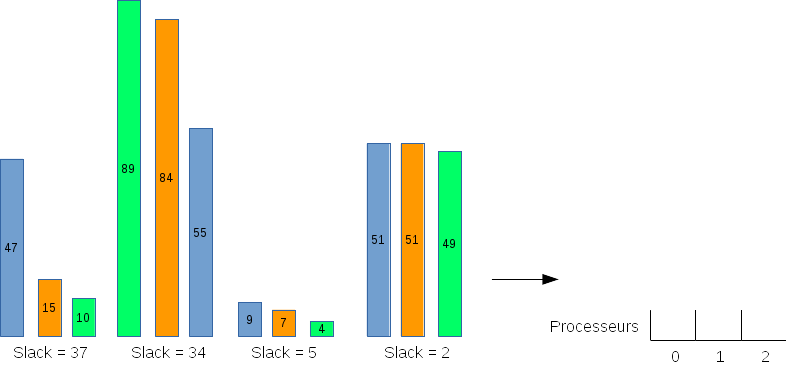
\includegraphics[width=\columnwidth]{Slack_Non_Unif_Exemple_Ok1.png}
\caption{Préparation des tuples pour SLACK avec $10\leq n \leq 1000$ et $5\leq m \leq 50$}
\label{ex:SLACKOK1}
\par}
\end{figure}

% FIGURE affectation des tuples
\begin{figure}
{\centering
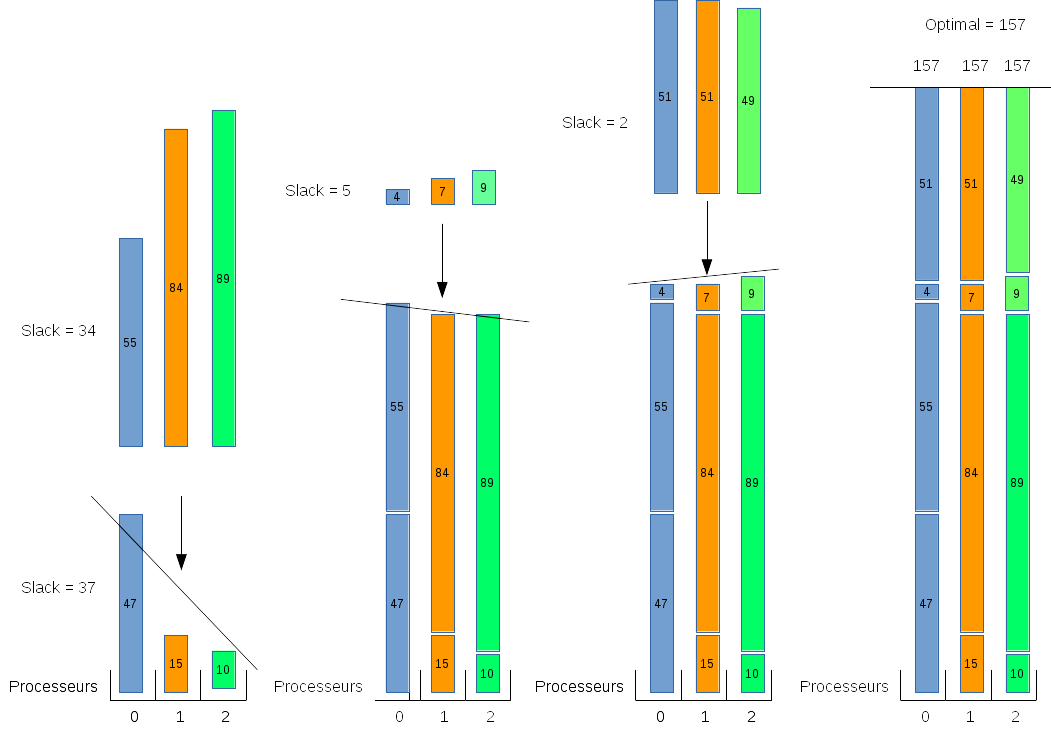
\includegraphics[width=\columnwidth]{Slack_Non_Unif_Exemple_Ok2.png}
\caption{Ordonnancement des tâches par tuple avec $10\leq n \leq 1000$ et $5\leq m \leq 50$}
\label{ex:SLACKOK2}
\par}
\end{figure}

Soit la liste de temps déjà ordonnée $$P = \{86, 83, 76, 75, 67, 44, 41, 26, 18, 5, 4, 3\}$$ à ordonnancer sur 3 machines. Ce qui donne les tuples ordonnés suivants (figure \ref{ex:SLACKOK1}):
\begin{itemize}
	\item $T_1$ $=\{75, 67, 44\}$, slack = 31;
	\item $T_2$ $=\{41, 26, 18\}$, slack = 23;
	\item $T_3$ $=\{86, 83, 76\}$, slack = 10;
	\item $T_4$ $=\{5, 4, 3\}$, slack = 2.
\end{itemize}
\jb{Ça ne correspond pas à la figure}

Pour chaque tuple, chaque tâche est affectée à chaque processeur (figure \ref{ex:SLACKOK2}), ce qui abouti vers une répartition équilibrée de temps par machine. Le Makespan est égale à l'optimal

\end{example}

Par contre si un job a un temps qui perturbe cette stratégie. Comme par exemple le premier job du deuxième tuple qui a un temps inférieur au slack du premier tuple. 
\jb{Manque des verbes dans les phrases précédentes}
Plus formellement si dans 
$$P = \{p_1, \ldots, p_m\}, \{p_{m+1}, \ldots, p_{2m}\}, \ldots, \{p_{n-m}, \ldots p_n\}$$
nous avons $p_{m+1} < p_m - p_1$, à l’opération du deuxième tuple, 2 jobs serons affectés au même processeur. Ce qui aura comme effet de déstabiliser l'harmonie des affectations des jobs de chaque tuple à chaque processeur et de provoquer un décalage entre l'optimal et le Makespan.

 

%--------------------------------------------------------
% EXEMPLE SLACK NON IDEAL
%--------------------------------------------------------
\begin{example}
Déroulement de SLACK dans un environnement non idéal.

% FIGURE des tuples
\begin{figure}
{\centering
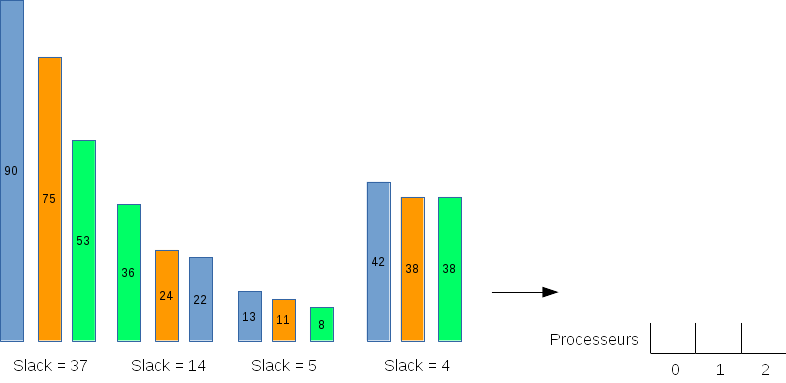
\includegraphics[width=\columnwidth]{Slack_Non_Unif_Exemple_PasOk1.png}
\caption{préparation des tuples pour SLACK avec $10\leq n \leq 1000$ et $5\leq m \leq 50$}
\label{ex:SLACKPasOK1}
\par}
\end{figure}

% FIGURE affectation des tuples
\begin{figure}
{\centering
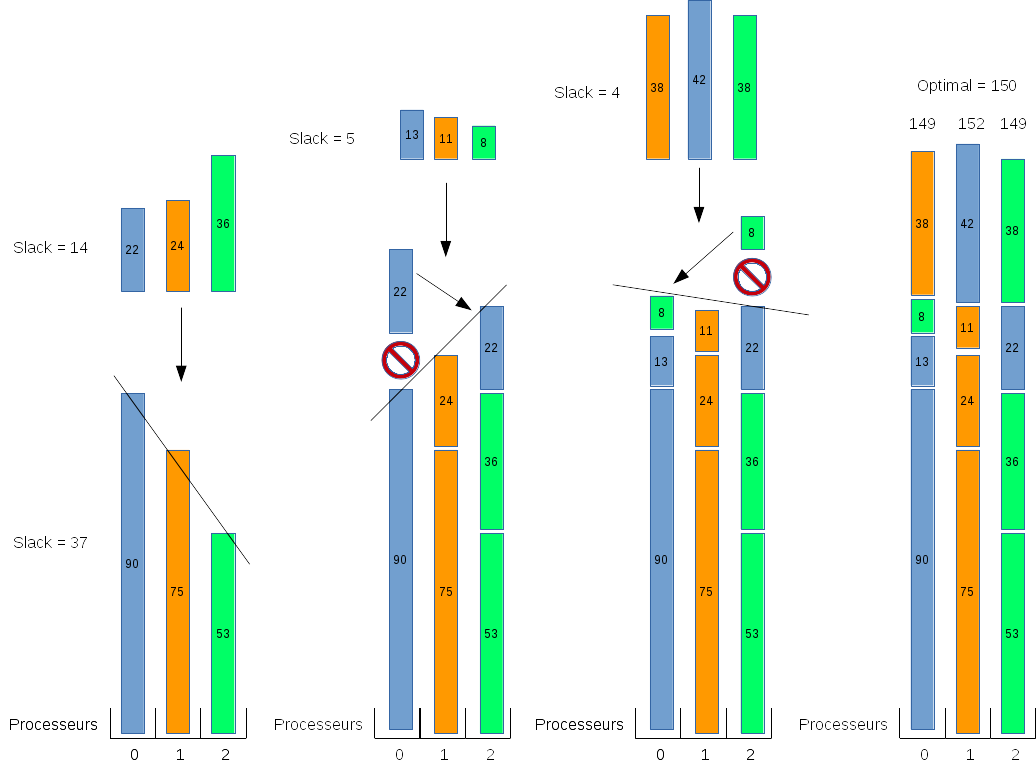
\includegraphics[width=\columnwidth]{Slack_Non_Unif_Exemple_PasOk2.png}
\caption{Ordonnancement des tâches par tuple avec $10\leq n \leq 1000$ et $5\leq m \leq 50$}
\label{ex:SLACKPasOK2}
\par}
\end{figure}

 
Soit la liste de temps déjà ordonnée $$P = \{90, 75, 53, 42, 38, 38, 36, 24, 22, 13, 11, 8\}$$ à ordonnancer sur 3 machines. Ce qui donne les tuples oordonnés suivants
\begin{itemize}
	\item $T_1$ $=\{90, 75, 53\}$, slack = 37;
	\item $T_2$ $=\{36, 24, 22\}$, slack = 14;
	\item $T_3$ $=\{13, 11, 8\}$, slack = 5;
	\item $T_4$ $=\{42, 38, 38\}$, slack = 4.
\end{itemize}
(figure \ref{ex:SLACKPasOK1}
Le premier job de $p_{T_2 1}=36 < slack(T_1)=37$ \lp{PB notation du
  job ?}
Après l'affectation de $T_1$ nous avons la répartition des charges des 
 processeurs suivante $\{(90), (75), (53)\}$.
Puis vient l'affectation de $T_2$, avec en premier le job $p_{T_2 1}=36$
nous avons la répartition des charges des processeurs suivante $\{(90), (75), (89 : 53,36)\}$. Le troisième processeur vient d'être chargé mais son poids $(89)$ est toujours inférieur au premier processeur $(90)$. Ce qu'aucun job de ce tuple ne sera affecté au premier processeur cette fois-ci (figure \ref{ex:SLACKPasOK2}).

Cette perturbation va se propager jusqu’à la fin de l'algorithme. Et le Makespan trouvé sera différent de l'optimal. 
\end{example}

Dans une liste de temps de type NON-UNIFORME de paramètres [a, b] le slack maximum possible 
  est égal à $slack_{max} = 0.9(b-a)$. 
Pour perturber le fonctionnement de SLACK, il faudrait une valeur de temps inférieure à $slack_{max}$. 
Or une liste de temps NON-UNIFORME ne contient aucune valeur comprise entre $0.9(b-a)$ et $0.2(b-a)$ 
  et seulement $2\%$ des éléments de la liste sont inférieurs à $0.2(b-a)$.
Ce qui réduit presque à $0$ les possibilités de générer une valeur qui peut potentiellement perturber SLACK.


Tester SLACK dans une instance de type NON-UNIFORME oriente le résultat d'efficacité.
           
\lp{La question qui se pose est: est-ce que les instances réelles sont
NON-UNIFORMES ?}


\section{Discussion} \label{sec:discussion}

SLACK, est plus efficace que LPT suivant 13 points de tests 
  dans un protocole expérimental. 
Mais il suffit de sortir de ce périmètre pour obtenir 
  une conclusion différente. 
Della Croce et Scatamacchia ont utilisé et combiné des variables 
  soit, trop différentes pour sortir un schéma de causalité pertinent, 
  soit pas assez représentatives pour en déduire un comportement général.  
En effet, certains points où SLACK est très efficace ont masqués 
  d'autres résultats où SLACK est moins percutant. 
Nous nous retrouvons devant un échantillon de tests biaisé et ne pouvons pas affirmer, même sur une distribution NON-UNIFORME, que SLACK améliore LPT. 

Au delà de ce problème, se pose la question : comment tester une heuristique par rapport à d'autres heuristiques par l'expérimentation ?
D'un point de vue théorique, ces heuristiques ont un ratio d'approximation, 
  une complexité en temps, voire un comportement asymptotique. 
Mais le ratio d’approximation n’est qu'une indication prouvée existante 
  à un instant donné, et prévaut tant qu'un nouveau ratio d'approximation 
  plus proche de l'optimal n'est pas trouvé et/ou prouvé. 
Même, si entre 2 heuristiques dont l'une à un ratio d'approximation 
  supérieur à l'autre, cette heuristique supposée théoriquement moins 
  efficace peut obtenir de meilleurs résultats par l'expérience.      
Le principe de randomisation est essentiel pour créer des échantillons servant 
  de support expérimental. 
Or un algorithme, comparé à d'autres, qui présente de meilleurs résultats 
  sur une distribution supposée perturber le comportement de toute heuristique 
  ne peut pas être gratifié d'algorithme améliorant un autre algorithme, 
  car il peut devenir mauvais sur une autre distribution. 
Pour tester une heuristique et en extraire une conclusion catégorique, 
  il faudrait la tester sur toutes distributions et combinaisons 
  de distributions, en faisant évoluer les paramètres de chacune d'elles 
 ($a$ et $b$ pour UNIFORME et NON UNIFORME, $\alpha$ et $\beta$ 
  pour les distributions Gamma et Beta $\ldots$), 
  et par rapport à une large variation de $n$ et $m$.  
Ce qui constitue un problème combinatoire.

Pour finir, lois stats sont inspirées de la nature  ..... alors pourquoi NON-UNIFORME ?

\section{Conclusion} \label{sec:conclusion}





\begin{appendices}

%\chapter{Génération des listes de nombres pseudo-aléatoires}

% \subsection{Objectifs}\label{ssec:synoptiqueObjectifs}

L'application doit permettre de reproduire un environnement expérimental d'exécution d'algorithmes liés au problème \problemGrahamP, et de les comparer entre eux au niveau de l'efficacité (borne d'approximation), et du coût en temps.
pour cela, il faut pouvoir :
\begin{itemize}
\item Générer des listes de temps de jobs selon différentes distributions et lois de probabilités, 
  afin de créer des instances (listes de temps de jobs~$+$~nombre de machines $m$) synthétiques. 
\item Récupérer des listes de temps existantes de chantiers réels disponibles au téléchargement, 
  permettant de créer des instances naturelles.
\item Caractériser ces listes de coûts de jobs, et ainsi estimer un niveau d’hétérogénéité 
  pour la mettre en relation avec le comportement des heuristiques.
\item Exécuter des heuristiques, récupérer leurs résultats (ordonnancement, Makespan) 
  et leur temps d’exécution 
  en fonction d'une liste de temps, et d'un nombre de machines $m$.
\item Exporter le résultats de plusieurs heuristiques soumises à 
  un environnement choisi 
  (instance, type  d'instance, variation du nombre de temps de jobs $n$, 
  variation du nombre de machines identiques $m$, algorithme utilisé) 
  dans le but de le soumettre à des scripts de statistiques et de comparaison (tableaux, graphes).
\item Archiver les différents résultats sous forme de données brutes, pour une utilisation future. 
\end{itemize} 
Pour finir, l'application se veut évolutive, et facilite, l'ajout d'heuristiques et de méthodes de générations de listes de temps.

% \subsection{Technologies utilisées}\label{ssec:synoptiqueTechnologiesUtilisées}

la partie applicative (génération d'instance, caractérisation des listes de temps, 
  exécution des algorithmes) est développée en PYTHON, et 
  la partie statistiques en langage R. 
Entre ces deux parties, les données brutes transitent via un fichier résultat au format CSV, 
 généré par le module PANDAS de PYTHON.
 
PYTHON et R ont été choisis pour les raisons suivantes :
\begin{itemize}
\item Temps de développement : ces langages, de haut niveau, permettent de développer 
  des solutions rapidement, avec une taille de code réduite.
\item Temps d'apprentissage : 
\item Se sont des langages interprètes : le fait que ces langages ne sont pas compilés 
  comprend plusieurs avantages. 
  D'une part, cela les rend (presque) indépendants des plate-formes d'exécution
  (la seule difficulté rencontrée, est l'adaptation à prévoir demeure dans la gestion des 
  chemins d'accès différente d'un OS à l'autre).
  D'autre part, les sources étant disponibles, cela permet une évolutivité de l’application. 
\item Les deux langages proposent des outils très efficaces permettant de travailler les listes.  
\item Abondances de bibliothèque : Il existe une multitude de bibliothèques permettant de 
  développer plus rapidement, 
  des fonctionnalités dans des domaines particuliers (mathématiques, statistiques, graphes, 
  structuration des données).

  e.g : 
  
  Pour PYTHON l'application utilise les bibliothèques 
  PANDAS (pour l'export des données data frame au format CSV) et 
  URLLIB (pour accéder au site de téléchargement et télécharger des listes de jobs existantes).

  Pour R, les scripts utilisent  
  READR (pour lire des fichiers CSV),  
  GGPLOT et PLOT3D (pour générer des graphes et les exporter au format PDF et JPG).
\item Ces plate-formes de développement sont gratuites. Ces langages sont donc largement utilisés 
  et la communauté est très active et productive,
  tant dans les tutoriels, 
  que dans les forums de discutions.         
\end{itemize}




\bigskip
Pour créer des listes de coûts, nous utilisons la bibliothèque par défaut de génération de 
  nombres pseudo-aléatoires de PYTHON, selon différentes règles statistiques. 
Ceci permet de créer des listes, pourvues de diverses propriétés, notamment l’hétérogénéité. 

\bigskip
Les deux types de générations suivants, implémentés dans l'application, 
  génèrent des nombres entiers \footnote{\samepage La commande random.uniform(a,b) de PYTHON renvoie un réel. L'application le transforme en entier, à l'aide de la commande round(n).}, mais ne permettent pas la maîtrise de la variance. 
Ce sont les deux seuls types de génération utilisés dans le protocole expérimental de comparaisons des heuristiques dans \cite{della2020longest}.
   
\begin{itemize}
\item Uniforme : les nombres pseudo-aléatoires générés, sont uniformément répartis 
  entre deux entiers $a$ et $b$.
   
  \begin{lstlisting}[language=Python]
	for i in range(n):
		rand = random.uniform(a,b)
  \end{lstlisting}

\item Non-uniforme. définie en tant que ``NON-UNIF'' dans \cite{frangioni2004multi}. Cette méthode produit
  une liste de temps de traitements dont 
  $98\%$ des éléments sont uniformément répartis dans l’intervalle  $[0.9 (b-a), b]$, et 
  le reste ($2\%$) est uniformément réparti dans l'intervalle  $[a, 0.2 (b-a)]$.


  \begin{lstlisting}[language=Python]
	n98 = int((98*n) / 100)
	    a1 = 0.9*(b-a)
    	b1 = b
    	a2 = a
    	b2 = 0.2*(b-a)
		...
    	for i in range(n98):
       		rand = random.uniform(a1,b1)

    	...
    
    	for i in range(n-n98):
    		rand = random.uniform(a2,b2)
  \end{lstlisting}
  
\end{itemize}

\bigskip
L'application implémente d'autres type de générations, basés sur des lois statistiques (distribution). 
Celles-ci génèrent des nombres réels, et acceptent des paramètres qui ont un effet sur 
  ``l'écrasement'' des courbes représentant les distributions, 
  et entrent dans le calculs de la variance.

\begin{itemize}
\item Loi gamma : La loi gamma représente généralement des manifestions qui se déroulent dans le temps. Elle accepte deux paramètres $k$ (``alpha'' dans l'implémentation) qui affecte la forme, et $\Theta$ (``beta'' dans l’implémentation) qui affecte l'échelle.  
  \begin{lstlisting}[language=Python]
	for i in range(n):
    		rand = random.gammavariate(alpha,beta)
  \end{lstlisting}
\item Loi exponentielle : Cas particulier de la loi gamma. Elle représente la durée de vie d'un événement. Elle accepte un paramètre $\lambda$ (lambda dans l'implémentation) qui affecte l'échelle.  
  \begin{lstlisting}[language=Python]
	for i in range(n):
    		rand = random.expovariate(lambd)
  \end{lstlisting}

\item Loi beta. Accepte deux paramètres de forme (un pour l'implémentation), $\alpha$ (alpha dans l’implémentation) qui affecte la forme, et $\beta$ (toujours à 1 dans l'implémentation) qui affecte aussi la forme.
  \begin{lstlisting}[language=Python]
	for i in range(n):
    		rand = random.betavariate(alpha,1)
  \end{lstlisting}

\end{itemize}

\bigskip
%\paragraph{Seed} Chaque génération d'instance est accompagnée de la récupération d'une graine (seed). 
Chaque instance a sa propre graine, et est stockée aussi dans le fichier de résultats. 
Ainsi il est aisé de reproduire à l'identique une liste de coûts, en utilisant la même graine 
  lors de sa ré-génération. 
 
les calculs sont effectués via les bibliothèques ``scipy.stats'' (pour les moyennes géométrique 
  et harmoniques) et ``statistics'' de PYTHON.

Sont calculées et récupérées dans un champs tuple (évolutif) :


%\subsection{Implémentation des algorithmes}
%\label{ssec:ImplémentationAlgorithmes}
Tous les algorithmes (étudiés) sont implémentés dans algorithms.py. Les procédures, objets et méthodes directement liés à ceux-ci sont placés dans ScheduleManagment.py i.e ceux qui n'ont pas le même prototype (FFD().). 
Ces algorithmes sont structurés sur le même principe :
\begin{itemize}

\item Les paramètres en entrée :
	\begin{description}

	\item Une liste de coûts : soit l'ensemble des $p_i$. 
	sous la forme $[p_1, p_2, ... , p_n]$. 
	Cette liste n'est pas forcément triée car cela fait partie 
	de l'heuristique, et ce tri peut changer d'une stratégie à l'autre.
	
	\item un nombre de machines m.
	\end{description}

\item Mesure du temps d'exécution. L'heure de début, et l'heure de fin 
sont consignées dans des variables ``before'' et ``after''. 
le temps d'exécution est donc mesuré en minutes-secondes.

\item Calcul du temps théorique, en fonction de la complexité théorique 
en temps de l’algorithme, ainsi que de la taille de la liste des temps, 
et du nombre de machines.

\item Déroulement de l'heuristique.

\item Retour d'un object ``PSched'' contenant les informations suivantes :
	\begin{description}
	\item Le nom de l'algorithme.
	\item Le temps attendu.
	\item le Makespan calculé
	\item Le temps qui a été nécessaire
	\item L'ordonnancement, sous forme de liste.
	\end{description}
\end{itemize}

%\subsection{COMBINE}\label{ssec:COMBINE}

les problèmes de COMBINE 
l'algo approximatif (Do while et do until a son importance
Cu - Cl >= alpha A pas forcément ...
Condition d'arrêt n'integre pas le nombre de bin utilisées

\fco {Discuter avec Laurent/Louis-Claude/Julien de ce bug-si connu ou viens de moi}
!!! La borne supérieure  est donnée par LPT rule !!!
puis FFD est exécuté avec, c= borne supérieure + borne inférieure)/2. Or, si FFD est moins performant que LPT, le nombre de bin ne sera jamais égal au nombre de machines considéré. e.g si LPT( [p1,p2,...,pn]) sur m machines donne U, et FFD(U) donne V (avec V > U) FFD entre U et L (L<U) donnera au mieux V.....

COMBINE avec borne sup = 1.1Cmax(LPT), c'est ok

Corrections apportées
algorithme COMBINE
algorithme FFD

%\subsection{fonctions annexes}\label{ssec:fonctionsAnnexes}

Quelques mots sur les fonctions appelées par les algorithmes principaux et qui ont leurs importance.

\begin{itemize}
\item FFD \cite{rieck2010basic} (implémentation)
\item Partitions LDM
\end{itemize}


%\subsection{Génération d'une campagne}\label{ssec:generationCampagne}
Par choix de paramètres
Par exécution pré remplie
Par lecture d'une campagnes

%\subsection{Gestion des "seeds"}\label{ssec:gestionSeeds}
si doit reproduire les mêmes instances


%\subsection{Structure du fichier résultat}\label{ssec:StructureFichierResultat}

passage en revue des colonnes de leur provenance


%\section{Comparaison des résultats} \label{sec:comparaisonResultats}

Comparer des algo quand on ne connaît pas l'optimal
par rapport au meilleurs résultat

%\subsection{Normalisation du MakeSpan}
%\label{ssec:normalisationMakeSpan}

trouver la bonne normalisation qui ne biaise pas trop la comparaison.
Mackespan sous forme brute, voire normalisé avec Cmax-optiml donne une courbe  accidentée et pas très lisible

\fco {Discuter avec Laurent/Louis-Claude/Julien si comparaison par graphes, ou voir moindres carrés ou autre méthode}

\begin{itemize}
\item MakeSpan brut
\item MakeSpan - optimal ou meilleur résultat
\item MakeSpan / optimal ou meilleur résultat
\item MakeSpan / Moyenne de tâche par machine
\end{itemize}

%\subsection{Temps d'exécution} \label{ssec:tempsExécution}

 Le temps attendu est théorique et non absolu. i.e n log n ne donne pas un temps en minutes secondes.Le temps mesuré lui est donné en minutes secondes --> faire le lien entre estimation théorique et mesuré.
 
D'un algo a l'autre , Python est un langatge de haut niveau, donc pas évident. ce qui peut être comparé, c'est pour un même algo et faire varier N et/ou m. on compare les mêmes instructions....

faire un lien entre le théorique de une valeur pour comparer par la suite les résultats suivants
 
%\subsection{Graphes}\label{ssec:graphes}
%\fco {Discuter avec Laurent/Louis-Claude/Julien Libre et proposition de graphes, ou conduit}

Différents graphe à disposition
utilisation de ggplot
Modifier l'un d'eux
Abscisse 	= soit n
			= soit m
Couleurs = algorithme
pictogramme = méthode de génération instance (lambda, beta uniforme ...) 
taille = hétérogénéité ?? écart type ?? de l'instance



\end{appendices} 



\bibliographystyle{plain}				% NE PAS ENLEVER !!!!!!!!!!
\bibliography{Bibliographie}			% Utilise Bibliographie.bib


% =======================================================
% ABSTRACT/RESUME
% =======================================================
\clearpage

%\abstractname{}


\selectlanguage{english}
\section*{Abstract} \label{sec:abstract}
%\paragraph{Abstract}
.... when the brief is completed ...

\bigskip
\selectlanguage{french}
\section*{Résumé} \label{sec:resume}
%\paragraph{Résumé}
....une fois le mémoire terminé ...



\end{document}
